\startchapter{Analysis}
\label{chapter:analysis}
We analyze ATLAS data to search for events which contain a pair of $W$ bosons with one decaying to $l\nu$ and the other decaying to $q\bar{q}$, and with the pair consistent with having been produced by a new resonance denoted by $s$ (as described in Chapter 2 subsection 2.2). Following the centrally-performed reconstruction of ATLAS proton-proton collision data, we analyze the reconstructed physics objects to search for evidence of new physics in this mono-$s$ \rightarrow\:$WW$ semileptonic channel. This thesis focuses on the design of the most sensitive ``merged" signal region of the possible phase space of events, as well as the addition of two control regions to constrain the \ttbar background contribution. Other regions used to specify potential signal and the various types of background within the analysis, as well as still further regions used for control and for validation of the analysis, are described in more brief detail in order to provide context to decision-making and a fuller picture of the analysis.

\section{Cut and Count Analysis}
This analysis uses the ``cut and count" strategy to search for evidence of the signal model. In order to perform this search, we define a set of selection criteria to slice or ``cut" the data according to various event variables, such as the amount of missing transverse momentum. We choose these selection criteria in order to maximize the expected number of signal events, and minimize the expected number of standard model background events in the region, based on the MC simulated data. While designing the selection criteria, real ATLAS data is hidden, or blinded, in order to avoid biasing the selection. The final area of phase space defined by the selection criteria is known as the ``signal region". As the final stage of an analysis, the real ATLAS data can be compared with the simulated MC data, and a statistical conclusion can be reached about the likelihood of the existence of the signal model. The more signal and less background that are present in the signal region, the stronger the statistical evidence for existence of the beyond-SM signal channel will be.

In order to improve the accuracy of the analysis and reduce the uncertainty on the amount of predicted standard model background, a ``control region" may also be used. This is a region not overlapping with the signal region which is designed to have similar kinematic properties to signal events, but be more pure in one or more standard model backgrounds and much less rich in actual expected signal events. In this region, we can compare the number of MC simulated background events and ATLAS data events, and any differences provide additional information to correct and constrain the expected number of background events in the signal region.

\section{Analysis Strategy}
\label{section:ana_strat}
In this analysis, there are two analysis channels which are combined statistically during fitting. These channels are distinguished by the reconstruction of the dijet system from the hadronically-decaying $W$ boson, and are named the \merged channel and the \resolved channel. In the \merged channel, we reconstruct the dijet system with a single $R=1.0$ Track-Assisted-Reclustered (TAR) jet, which generally means that the dijet system is more boosted, with the $s$ decay products closer together. In the less-boosted \resolved channel we reconstruct the dijet system using a pair of $R=0.4$ jets. Figure \ref{fig:mgd_res} provides a visual demonstration of this difference. In each analysis channel there are three analysis regions: the semileptonic signal region, a control region designed to constrain the \ttbar background, and a control region designed to constrain the \wjets background. To ensure that \merged and \resolved regions do not overlap, an event recycling strategy is employed where only events failing the selection for all \merged regions are considered for selection in \resolved regions.

\begin{figure}[h!]
    \centering
    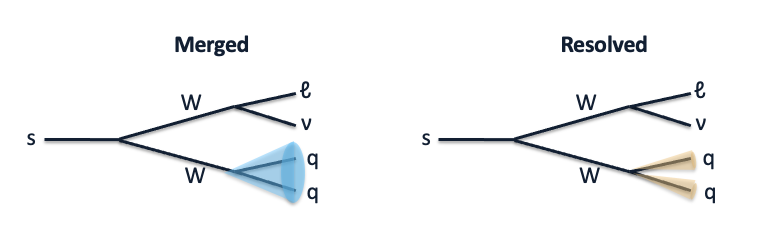
\includegraphics[width=0.8\textwidth]{Figures/4/mgd_res.png}
    \caption{Schematic representation of the differing reconstruction technique between merged and resolved regions.}
    \label{fig:mgd_res}
\end{figure}

\section{Merged Signal Region}
\label{section:sr_merged}
\subsection{Signal and Background Characterization}
The first step towards defining signal region selection criteria is to characterize signal and background events, while searching for exploitable differences. Event characteristics explored include the relative positions of analysis objects, the transverse momenta and masses of analysis objects, along with various jet substructure variables. Figures \ref{fig:Presel1}, \ref{fig:Presel2}, and \ref{fig:Presel3} in Appendix section \ref{section:preselection} show distributions of signal and background events for many of the variables studied at preselection level.

\subsection{TAR Jet Lepton Disentanglement}
Reconstructing the hadronically-decaying $W$ boson as accurately as possible is key in this analysis. As a result, it is given special attention, especially in the more sensitive merged channel. In this channel, the $W$ is reconstructed by a single $R=1.0$ TAR jet. Due to the boosted nature of the $s$-decay, however, the leptonically-decaying $W$ often lies in or very near to this jet. As a result, the charged lepton often overlaps the TAR jet, which can lead to difficulty in jet reconstruction.

In order to resolve this difficulty,wemade modifications to the TAR jet building process to disentangle overlapping leptons. We identify input tracks and jets that are likely to be attributable to a final state lepton and not the hadronic $W$ decay, and remove them. To achieve this, we remove tracks associated with a baseline electron or muon from the input track collection. We then also remove any \akt $R=0.2$ jet overlapping with a baseline electron (defined here as having $\Delta R(lep,jet) < 0.2$) prior to reclustering into $R=1.0$ jets. We do not remove $R=0.2$ jets overlapping muons, as muons do not leave large a calorimeter signature and are therefore unlikely to fake hadronic activity. This results in the following updated TAR jet building algorithm, where steps with a (*) are added to disentangle leptons:

\begin{itemize}
  \item Tracks and calibrated \akt $R=0.2$ jets are chosen as input to the algorithm.
  \item Tracks associated with a baseline muon or electron are removed from the input collection (*).
  \item \akt $R=0.2$ jets overlapping with a baseline electron ($\Delta R<0.2$) are removed from the input collection (*).
  \item The remaining \akt $R=0.2$ jets are reclustered into $R=1.0$ jets using the \akt algorithm, and trimmed using the $p_T$ fraction \(f_{cut}=0.05\).
  \item Input tracks are matched to $R=0.2$ jets if possible, using ghost association.
  \item Tracks which remain unassociated are matched to the nearest \akt $R=0.2$ jet within $\Delta R<0.3$.
  \item The \pT of each track is rescaled using the \pT of the jet to which it is matched using the equation:
  \begin{equation}
  \pT^{\text{track, new}} = \pT^{\text{track, old}}\times \frac{\pT^{\text{subjet $j$}}}{\sum_{i \in j} \pT^{\text{track $i$}}} ,
  \label{eq:TAR_rescale}
  \end{equation}  where $j$ is the $R=0.2$ subjet that the track being rescaled is matched with, and the index $i$ runs over all tracks matched to that subjet. This rescaling accounts for the momentum of neutral particles (except for neutrinos), which is measured at calorimeter level but is not visible in the tracker.
  \item Finally, jet substructure variables and  $m^\text{TAR}$ are calculated using the rescaled matched tracks.
\end{itemize}

In order to study the potential benefit of lepton-disentanglement, we produced near-identical sets of signal MC samples, with one implementing disentanglement and the other not.
We then compared the mass of the reconstructed jets in the two samples in a region where a lepton overlaps the $R=1.0$ TAR Jet $(\Delta R(e, \text{TAR}) < 1)$, to determine how well the $W$ boson mass is reconstructed in this case.
Figure \ref{fig:TARdisentaglementplots} demonstrates the improvement in mass resolution achieved by disentangling leptons from TAR jets. A clearly enhanced resolution in the TAR jet mass peak around the $W$ mass is visible for the lepton-disentangled jets in the electron channel. This significantly improves sensitivity in the merged signal region by allowing a much tighter selection on the TAR jet mass. Very little changes in the muon channel.

We additionally compared the performance of building the TAR jets from constituent \akt $R=0.4$ jets, rather than \akt $R=0.2$ jets.
In the electron channel we found that for high $s$ mass, $W$ mass reconstruction performance was similar between the two methods, but for low $s$ mass using \akt $R=0.4$ jets significantly impairs resolution around the $W$ mass.
Again in the muon channel we observed few significant differences.
Figure \ref{fig:R04_TAR_plots} shows a comparison of the TAR jet mass distribution built from \akt $R=0.4$ and \akt $R=0.2$ jets, for two selected signal points, in a signal-enriched region with 1 electron, $\Delta R(e, \text{TAR})< 1$, and $\mtlepmet > 150$~GeV. This clearly demonstrates the improved mass resolution for the signal point at $m_s = 160 $~GeV.
\begin{figure}[!h]
\centering
   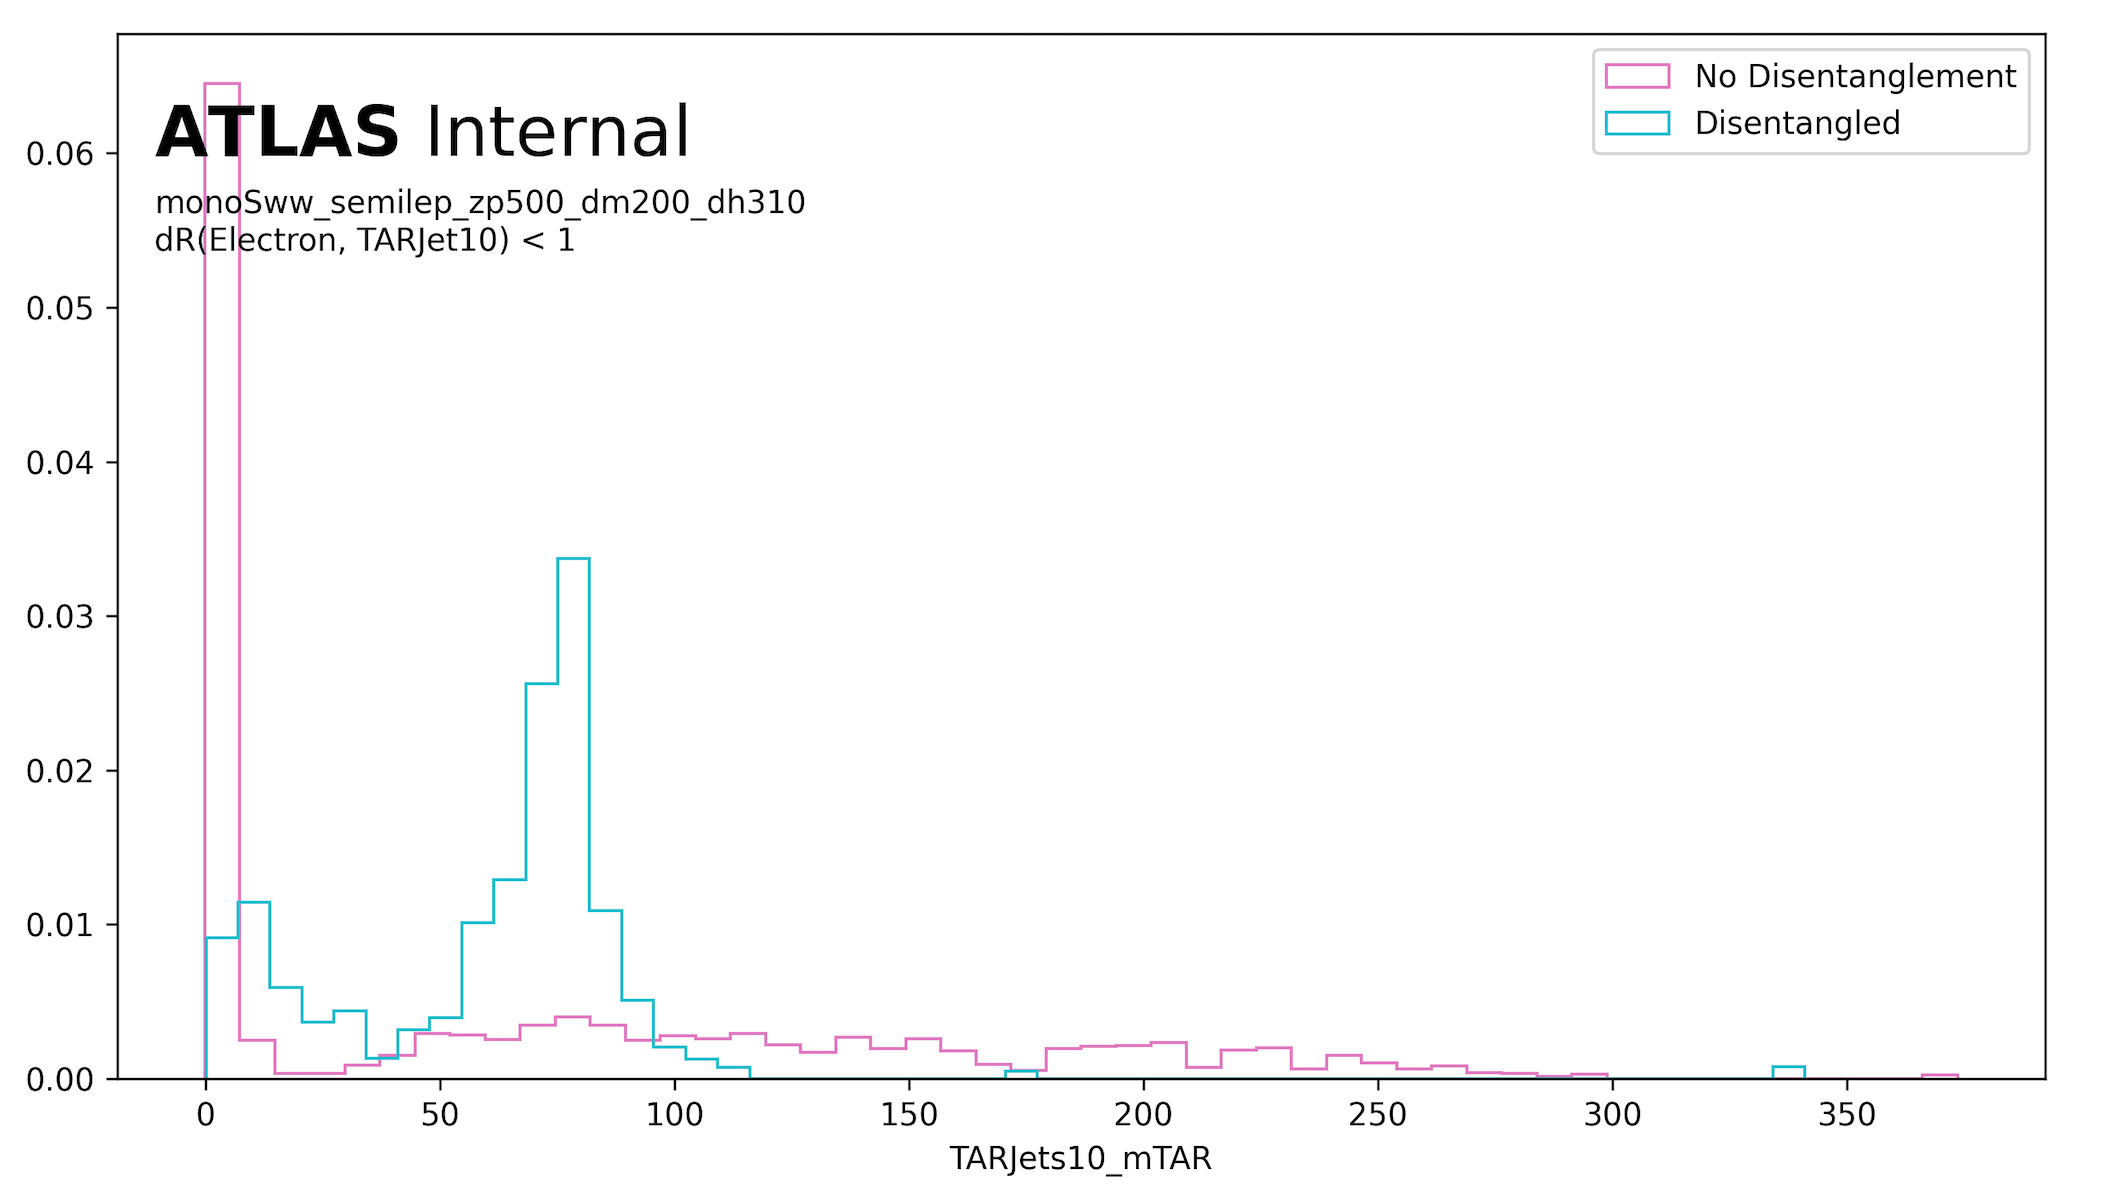
\includegraphics[width = 0.49\textwidth]{Figures/4/TAR/monoSww_semilep_zp500_dm200_dh310.png}
   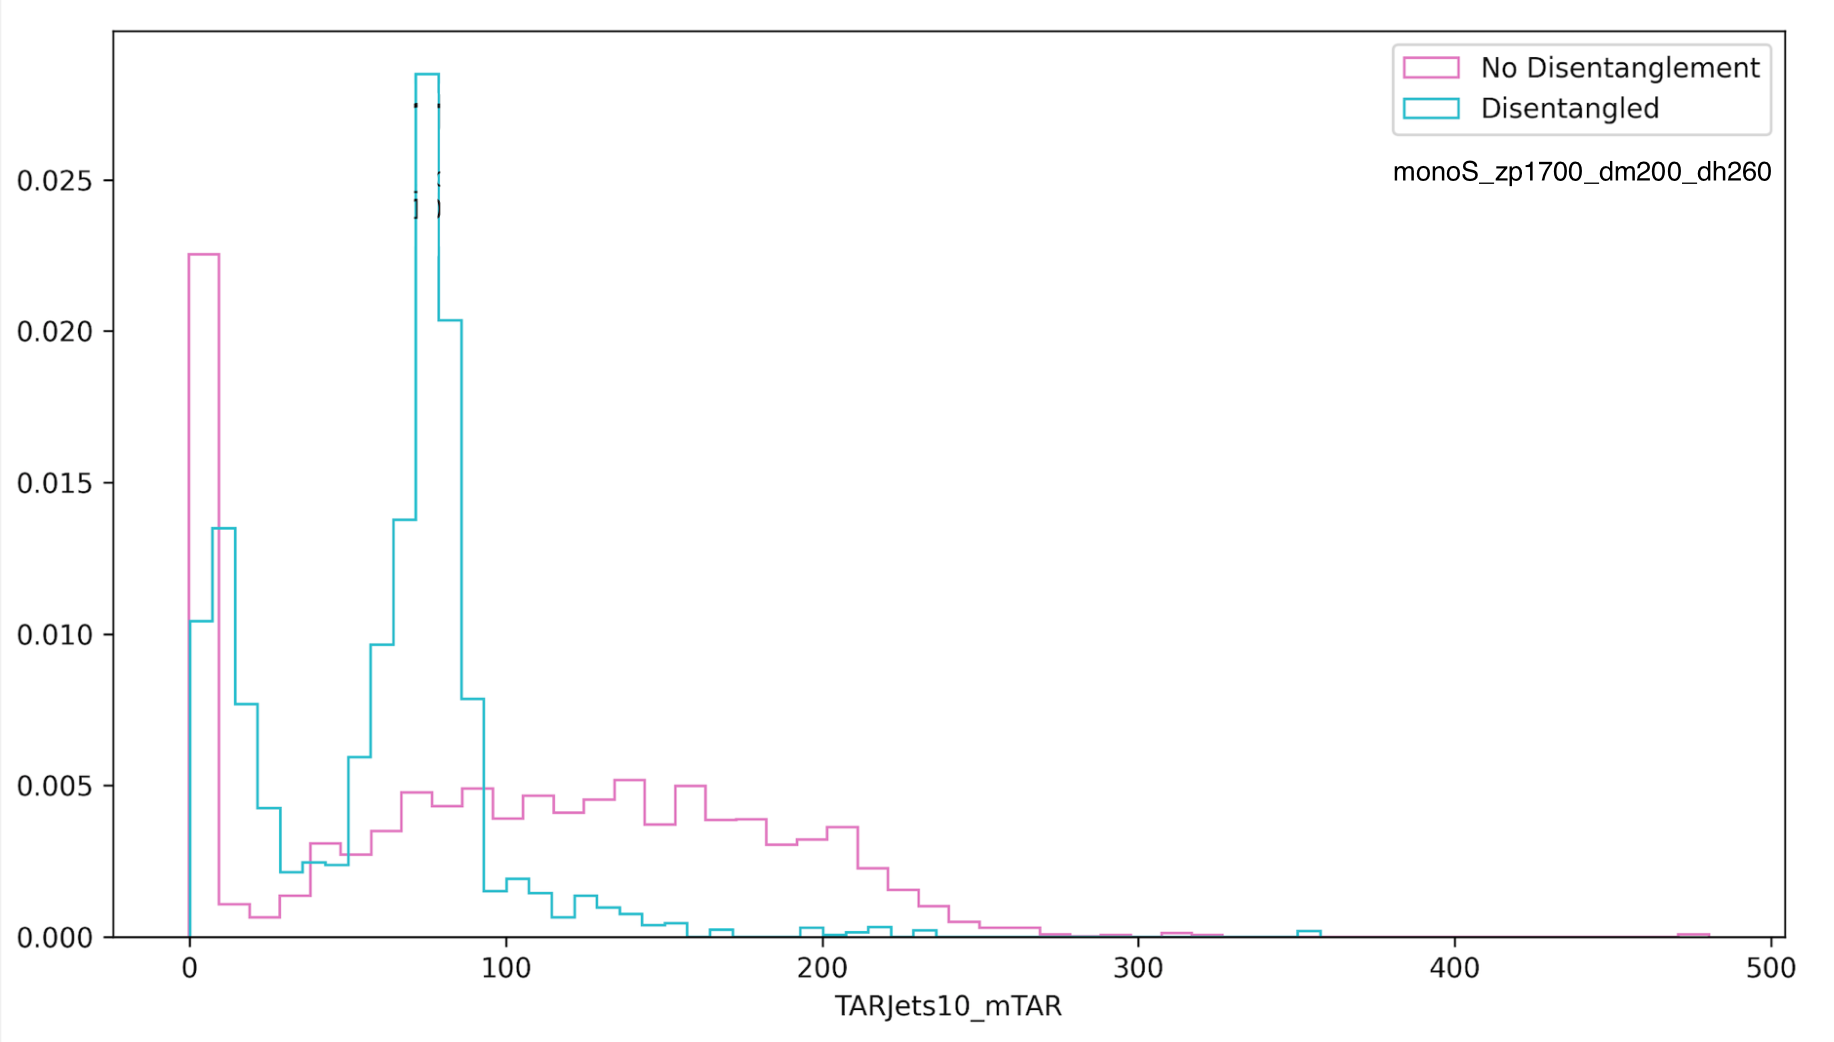
\includegraphics[width = 0.49\textwidth]{Figures/4/TAR/monoSww_semilep_zp1700_dm200_dh260.png}

   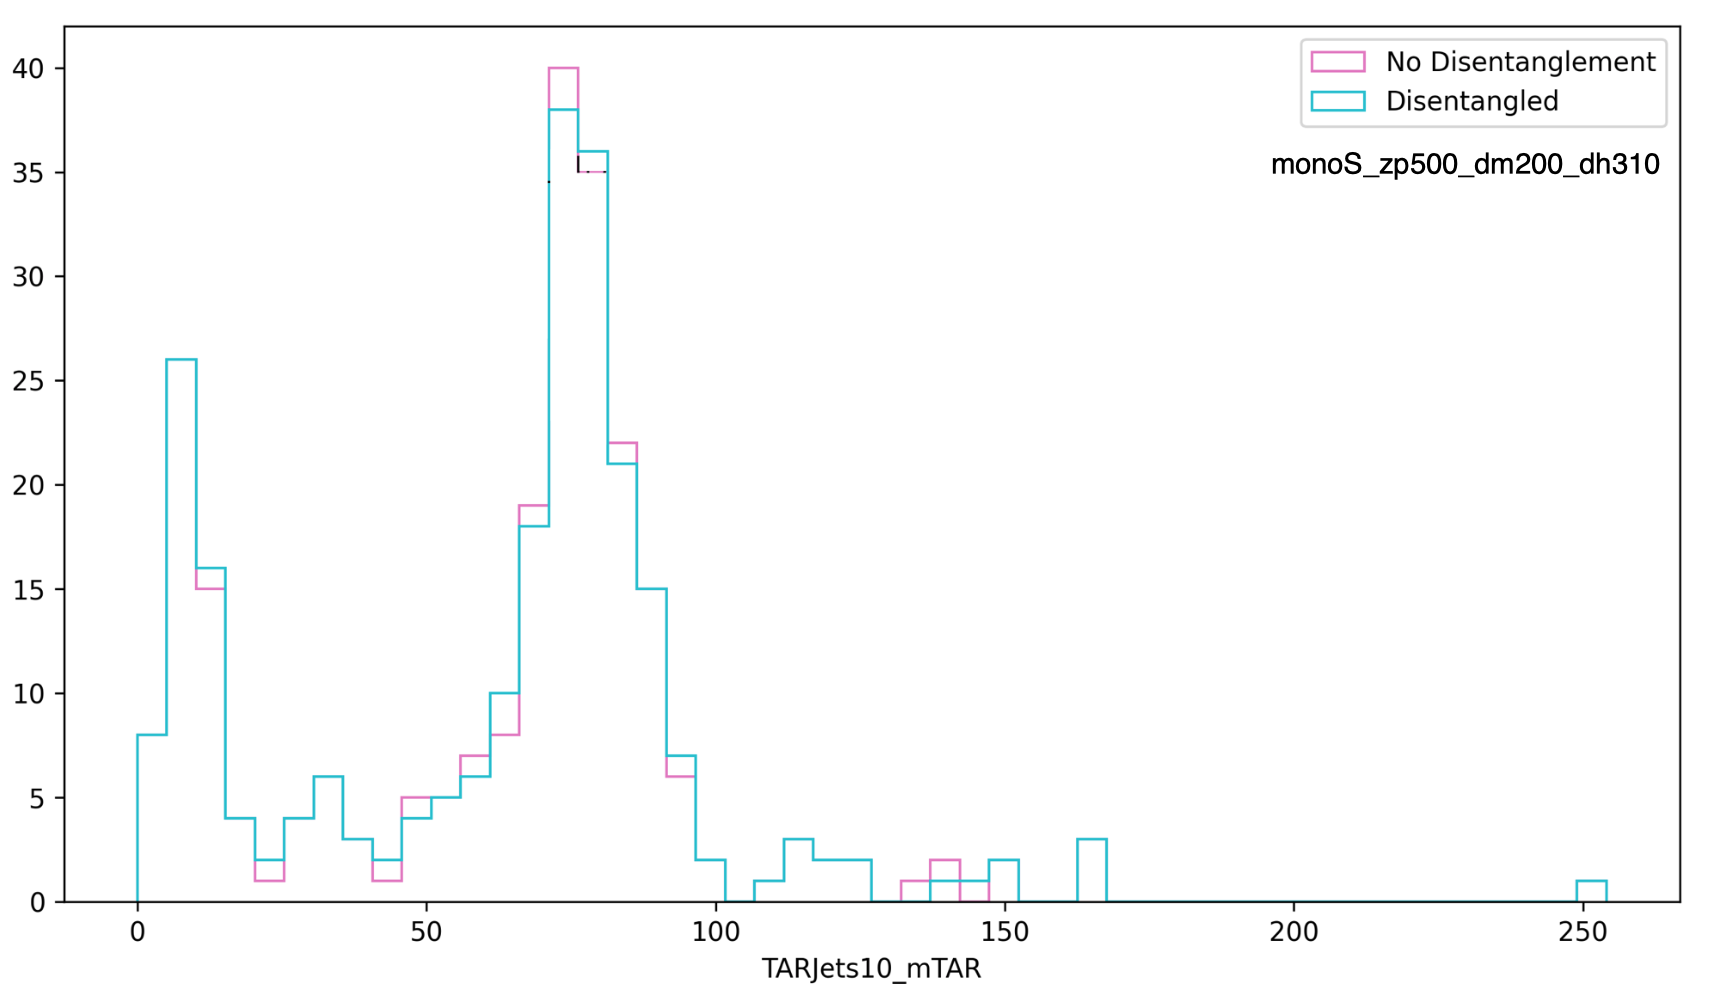
\includegraphics[width = 0.49\textwidth]{Figures/4/TAR/mu_monoSww_semilep_zp500_dm200_dh310.png}
   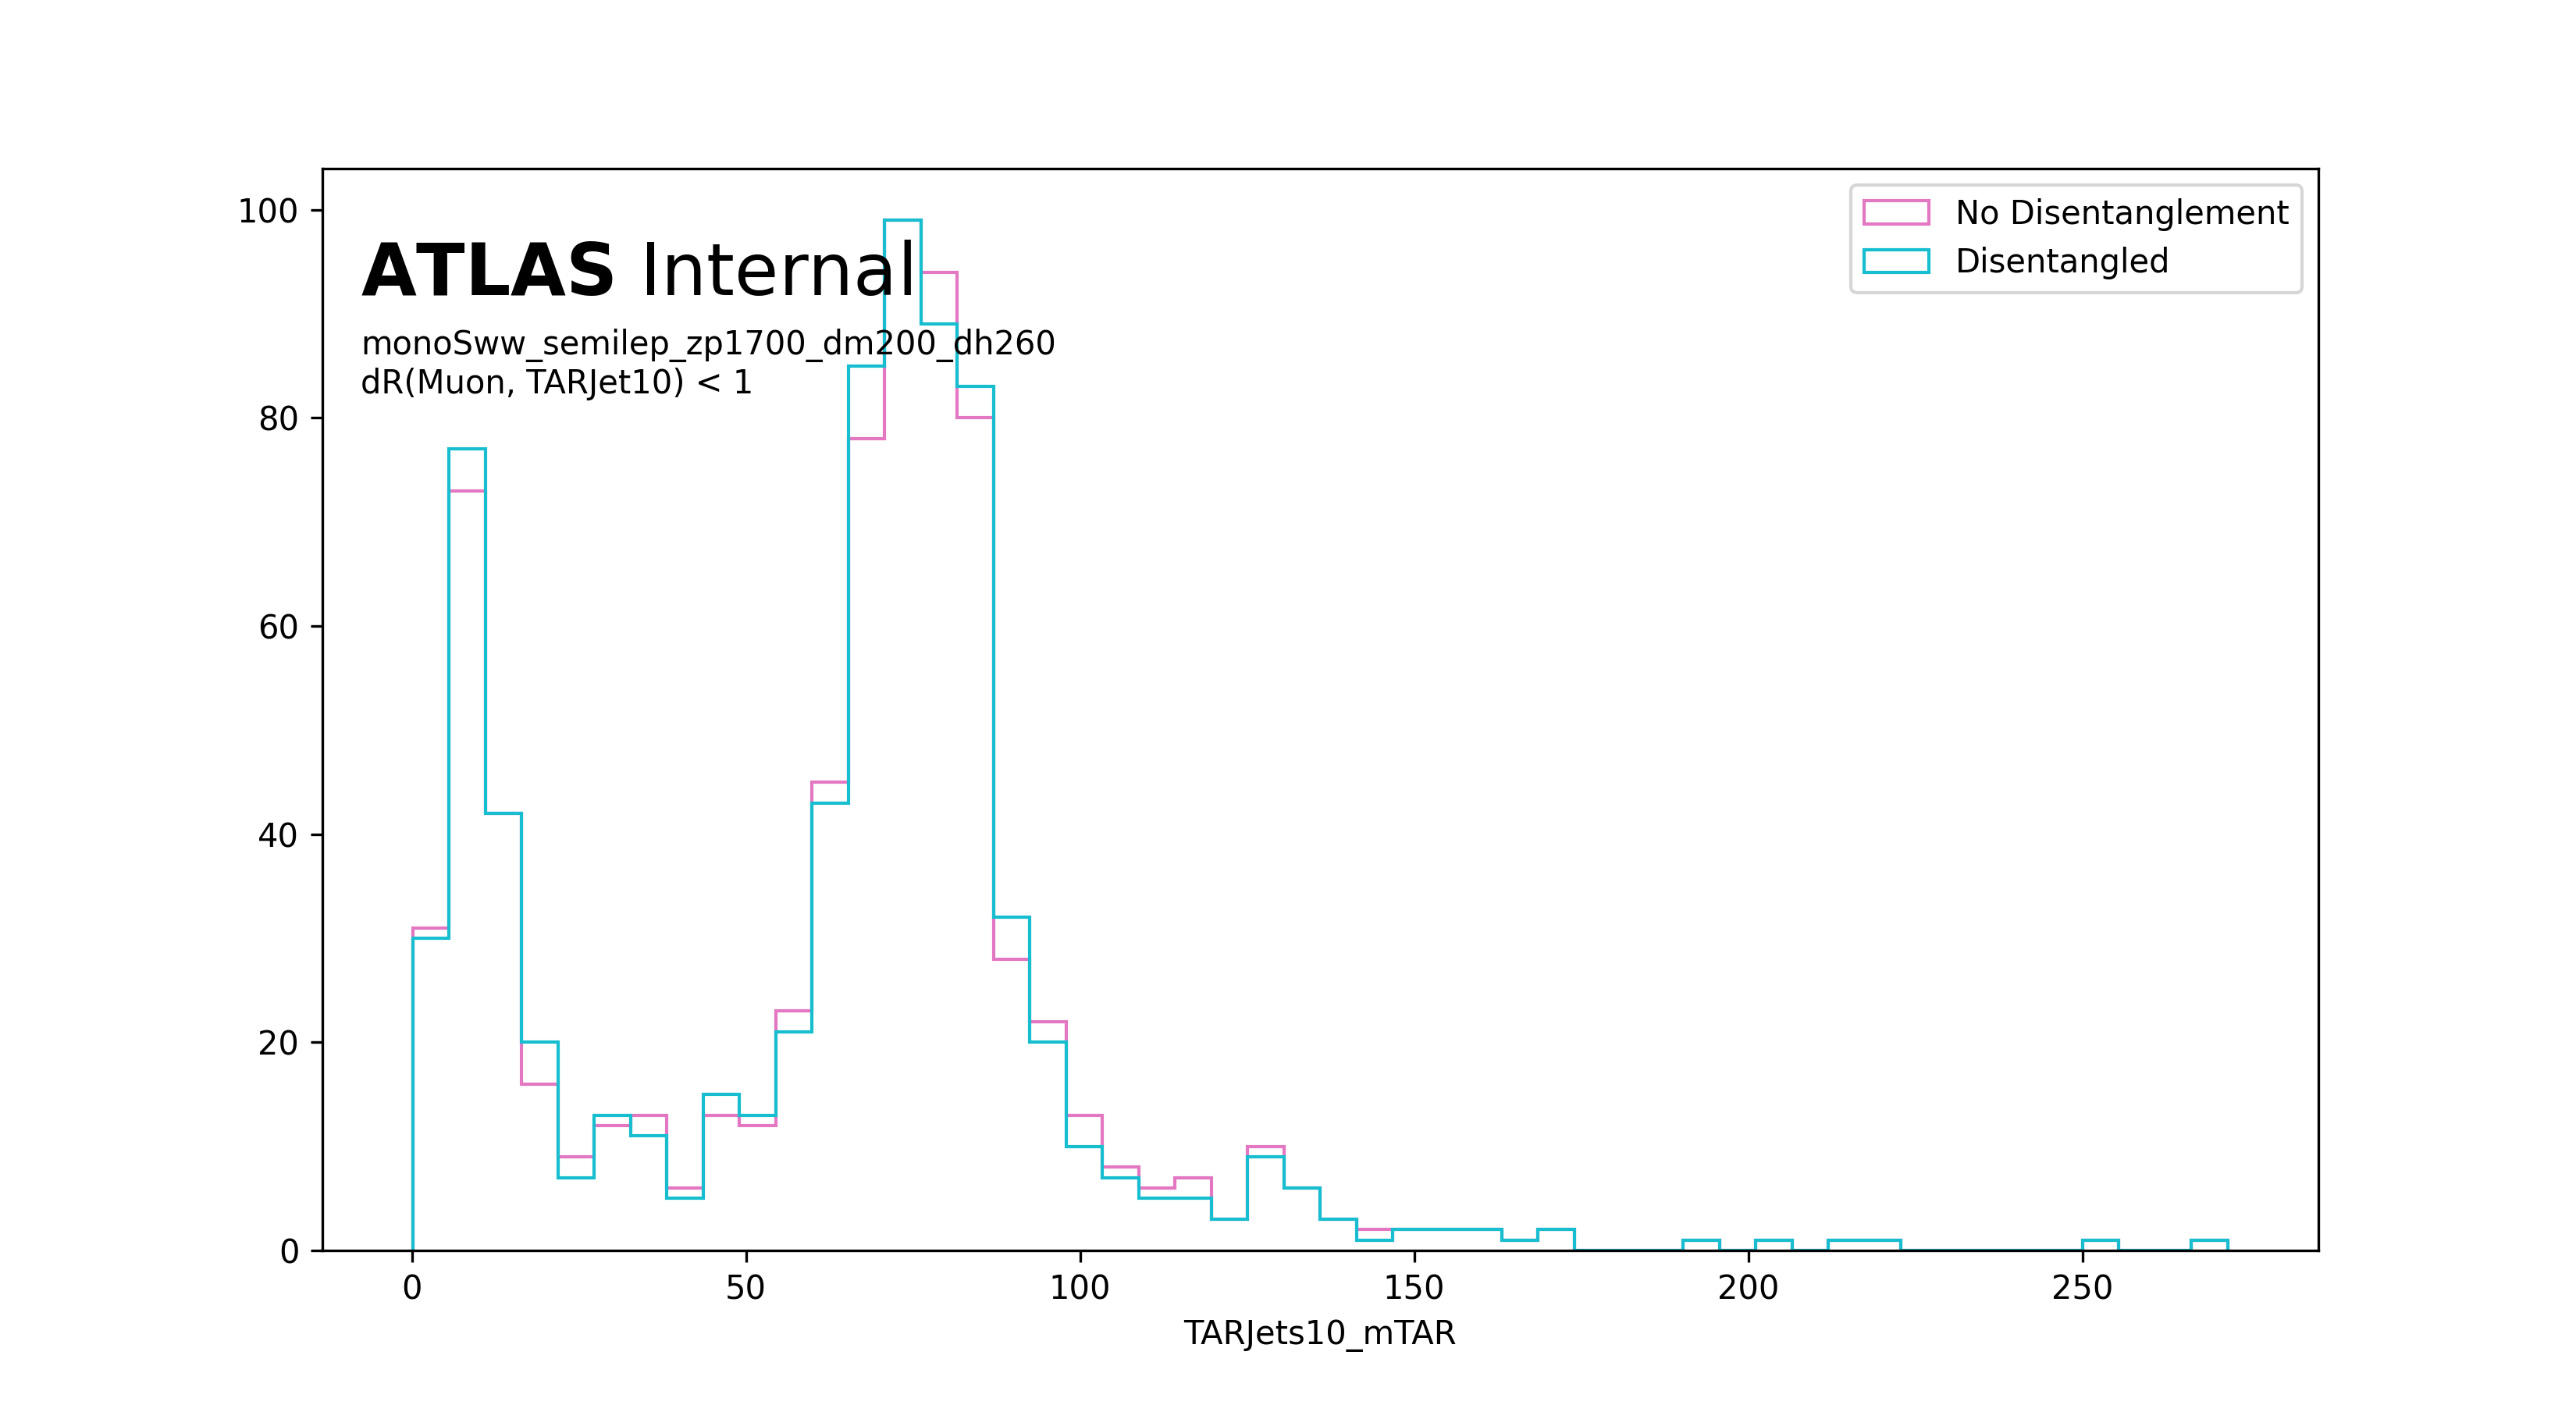
\includegraphics[width = 0.49\textwidth]{Figures/4/TAR/mu_monoSww_semilep_zp1700_dm200_dh260.png}

   \caption{Normalized $R=1.0$ TAR jet mass distributions with and without lepton disentanglement applied for four representative signal points. \textbf{Upper row:} electron channel, \textbf{lower row:} muon channel.}
   \label{fig:TARdisentaglementplots}
\end{figure}

\begin{figure}[h]
  \centering
     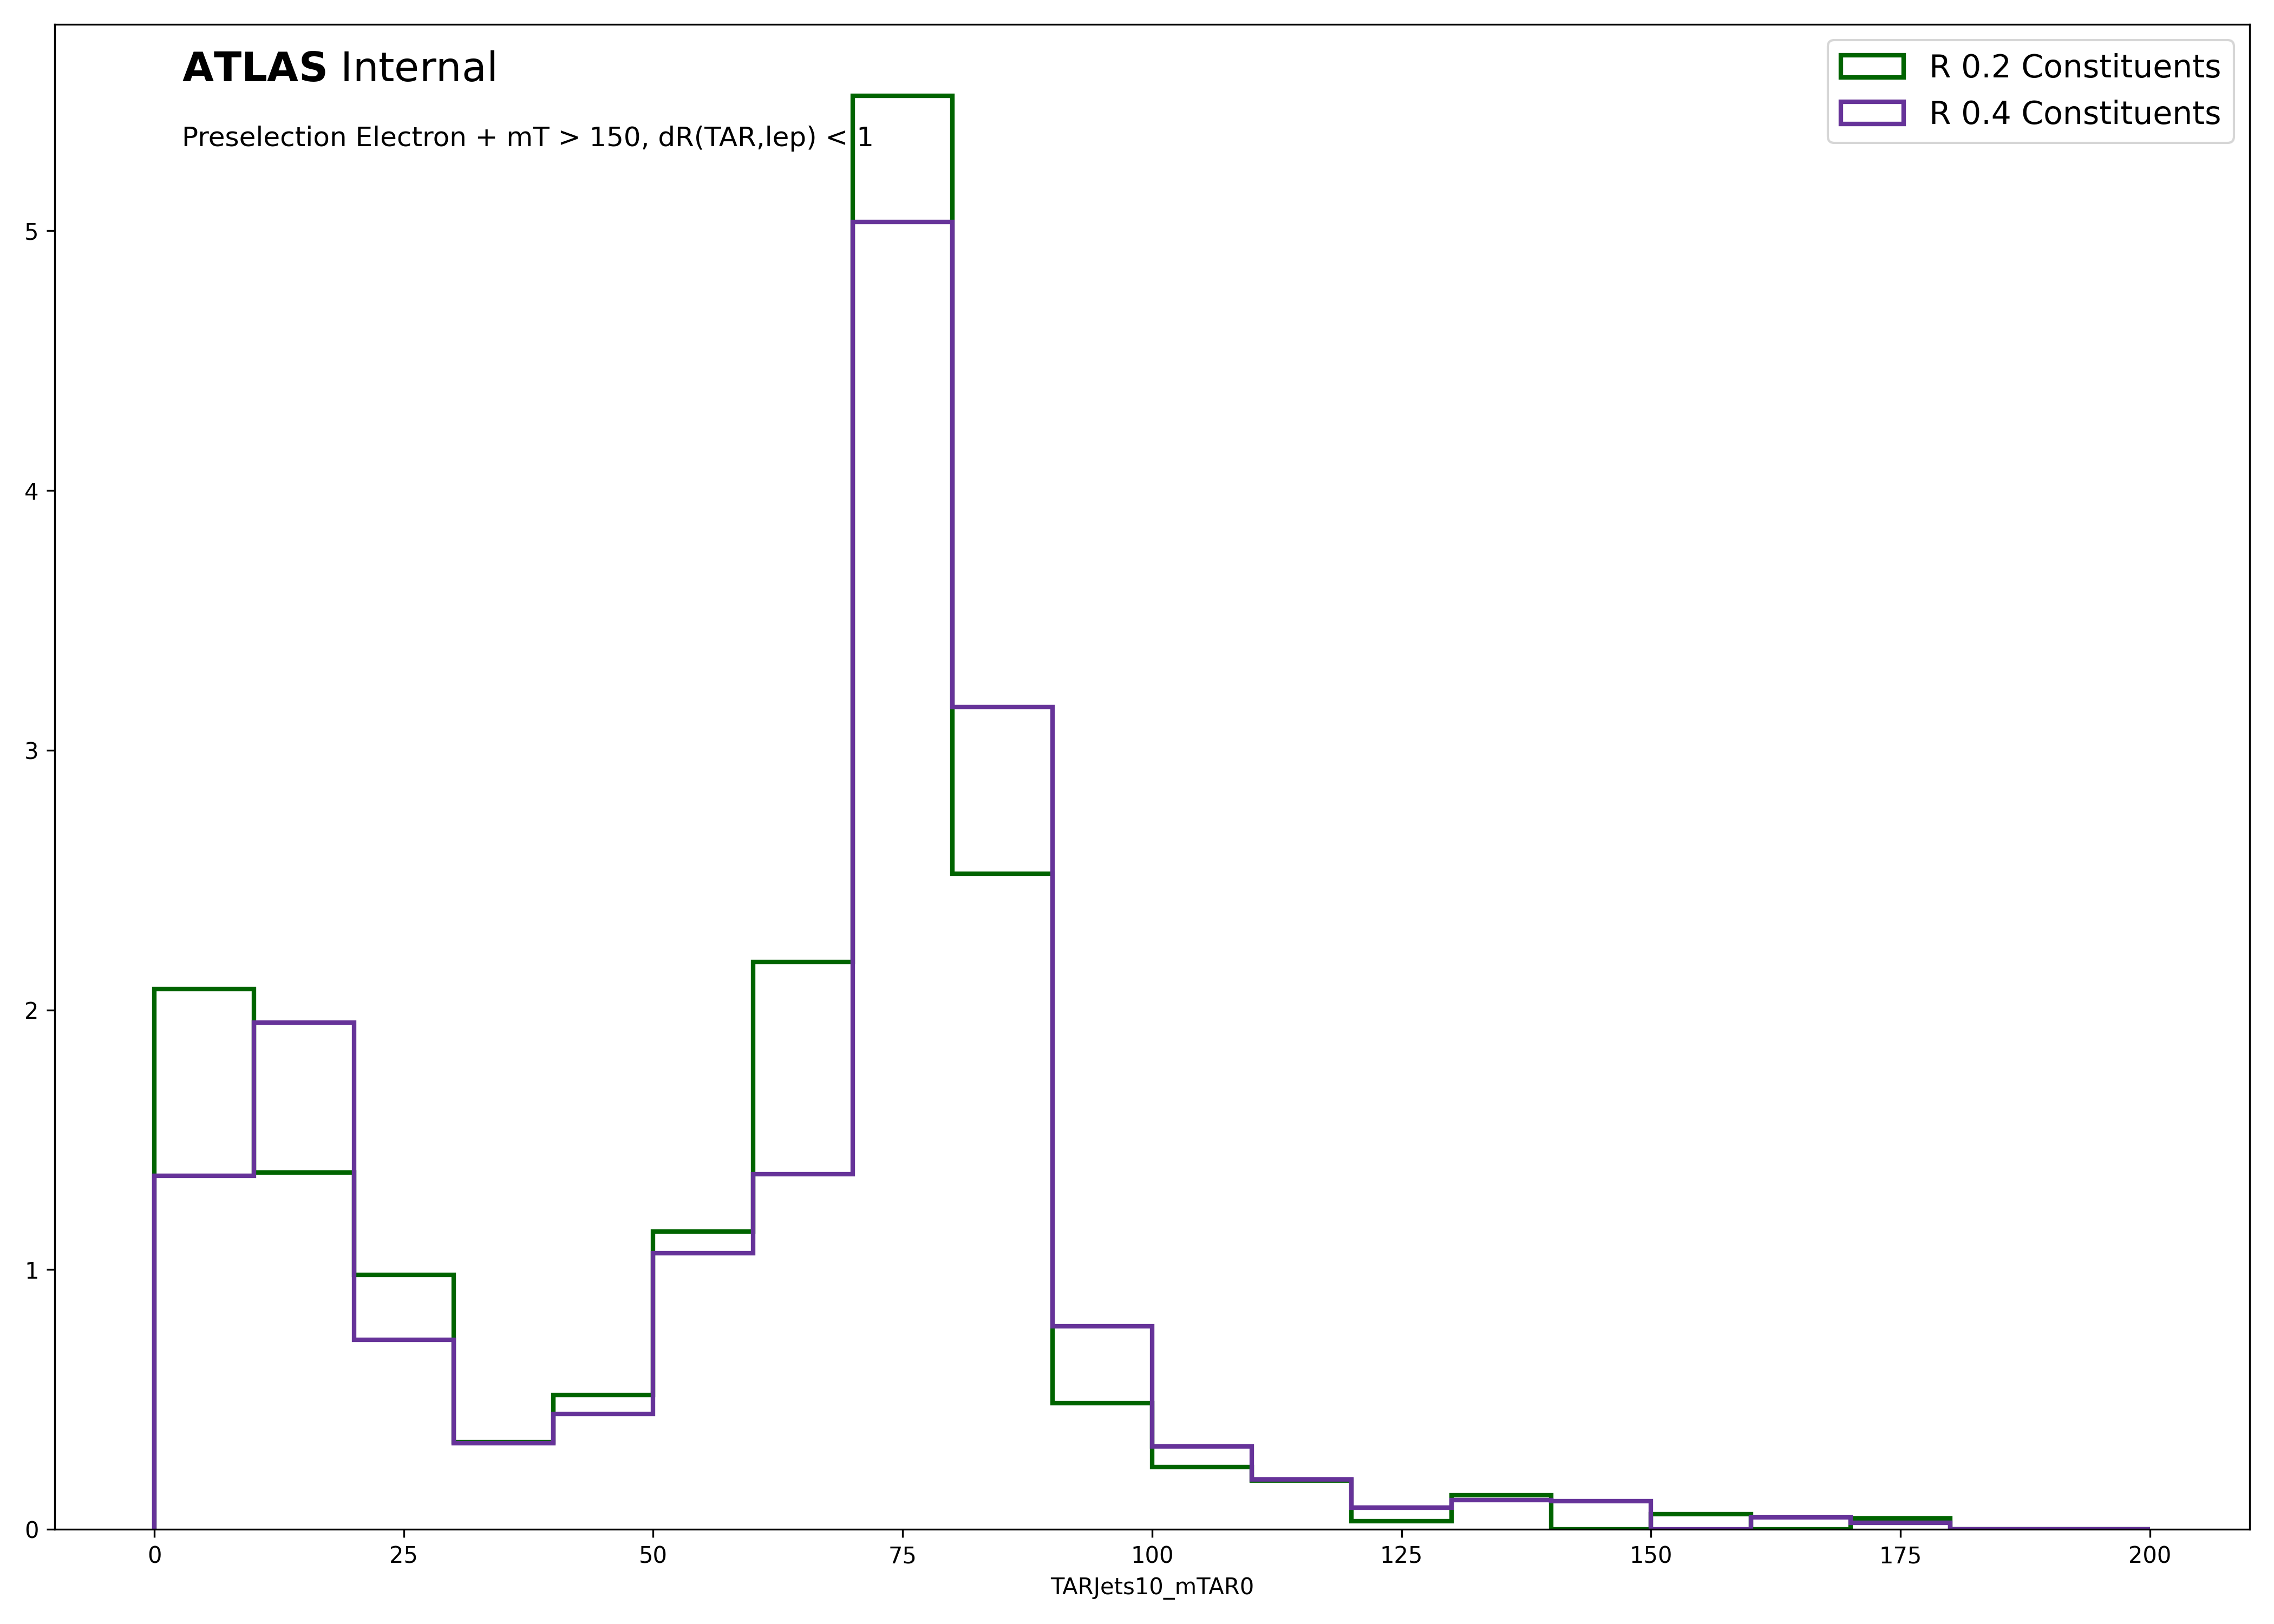
\includegraphics[width = 0.49\textwidth]{Figures/4/TAR/04_monoSww_semilep_zp500_dm200_dh310.png}
     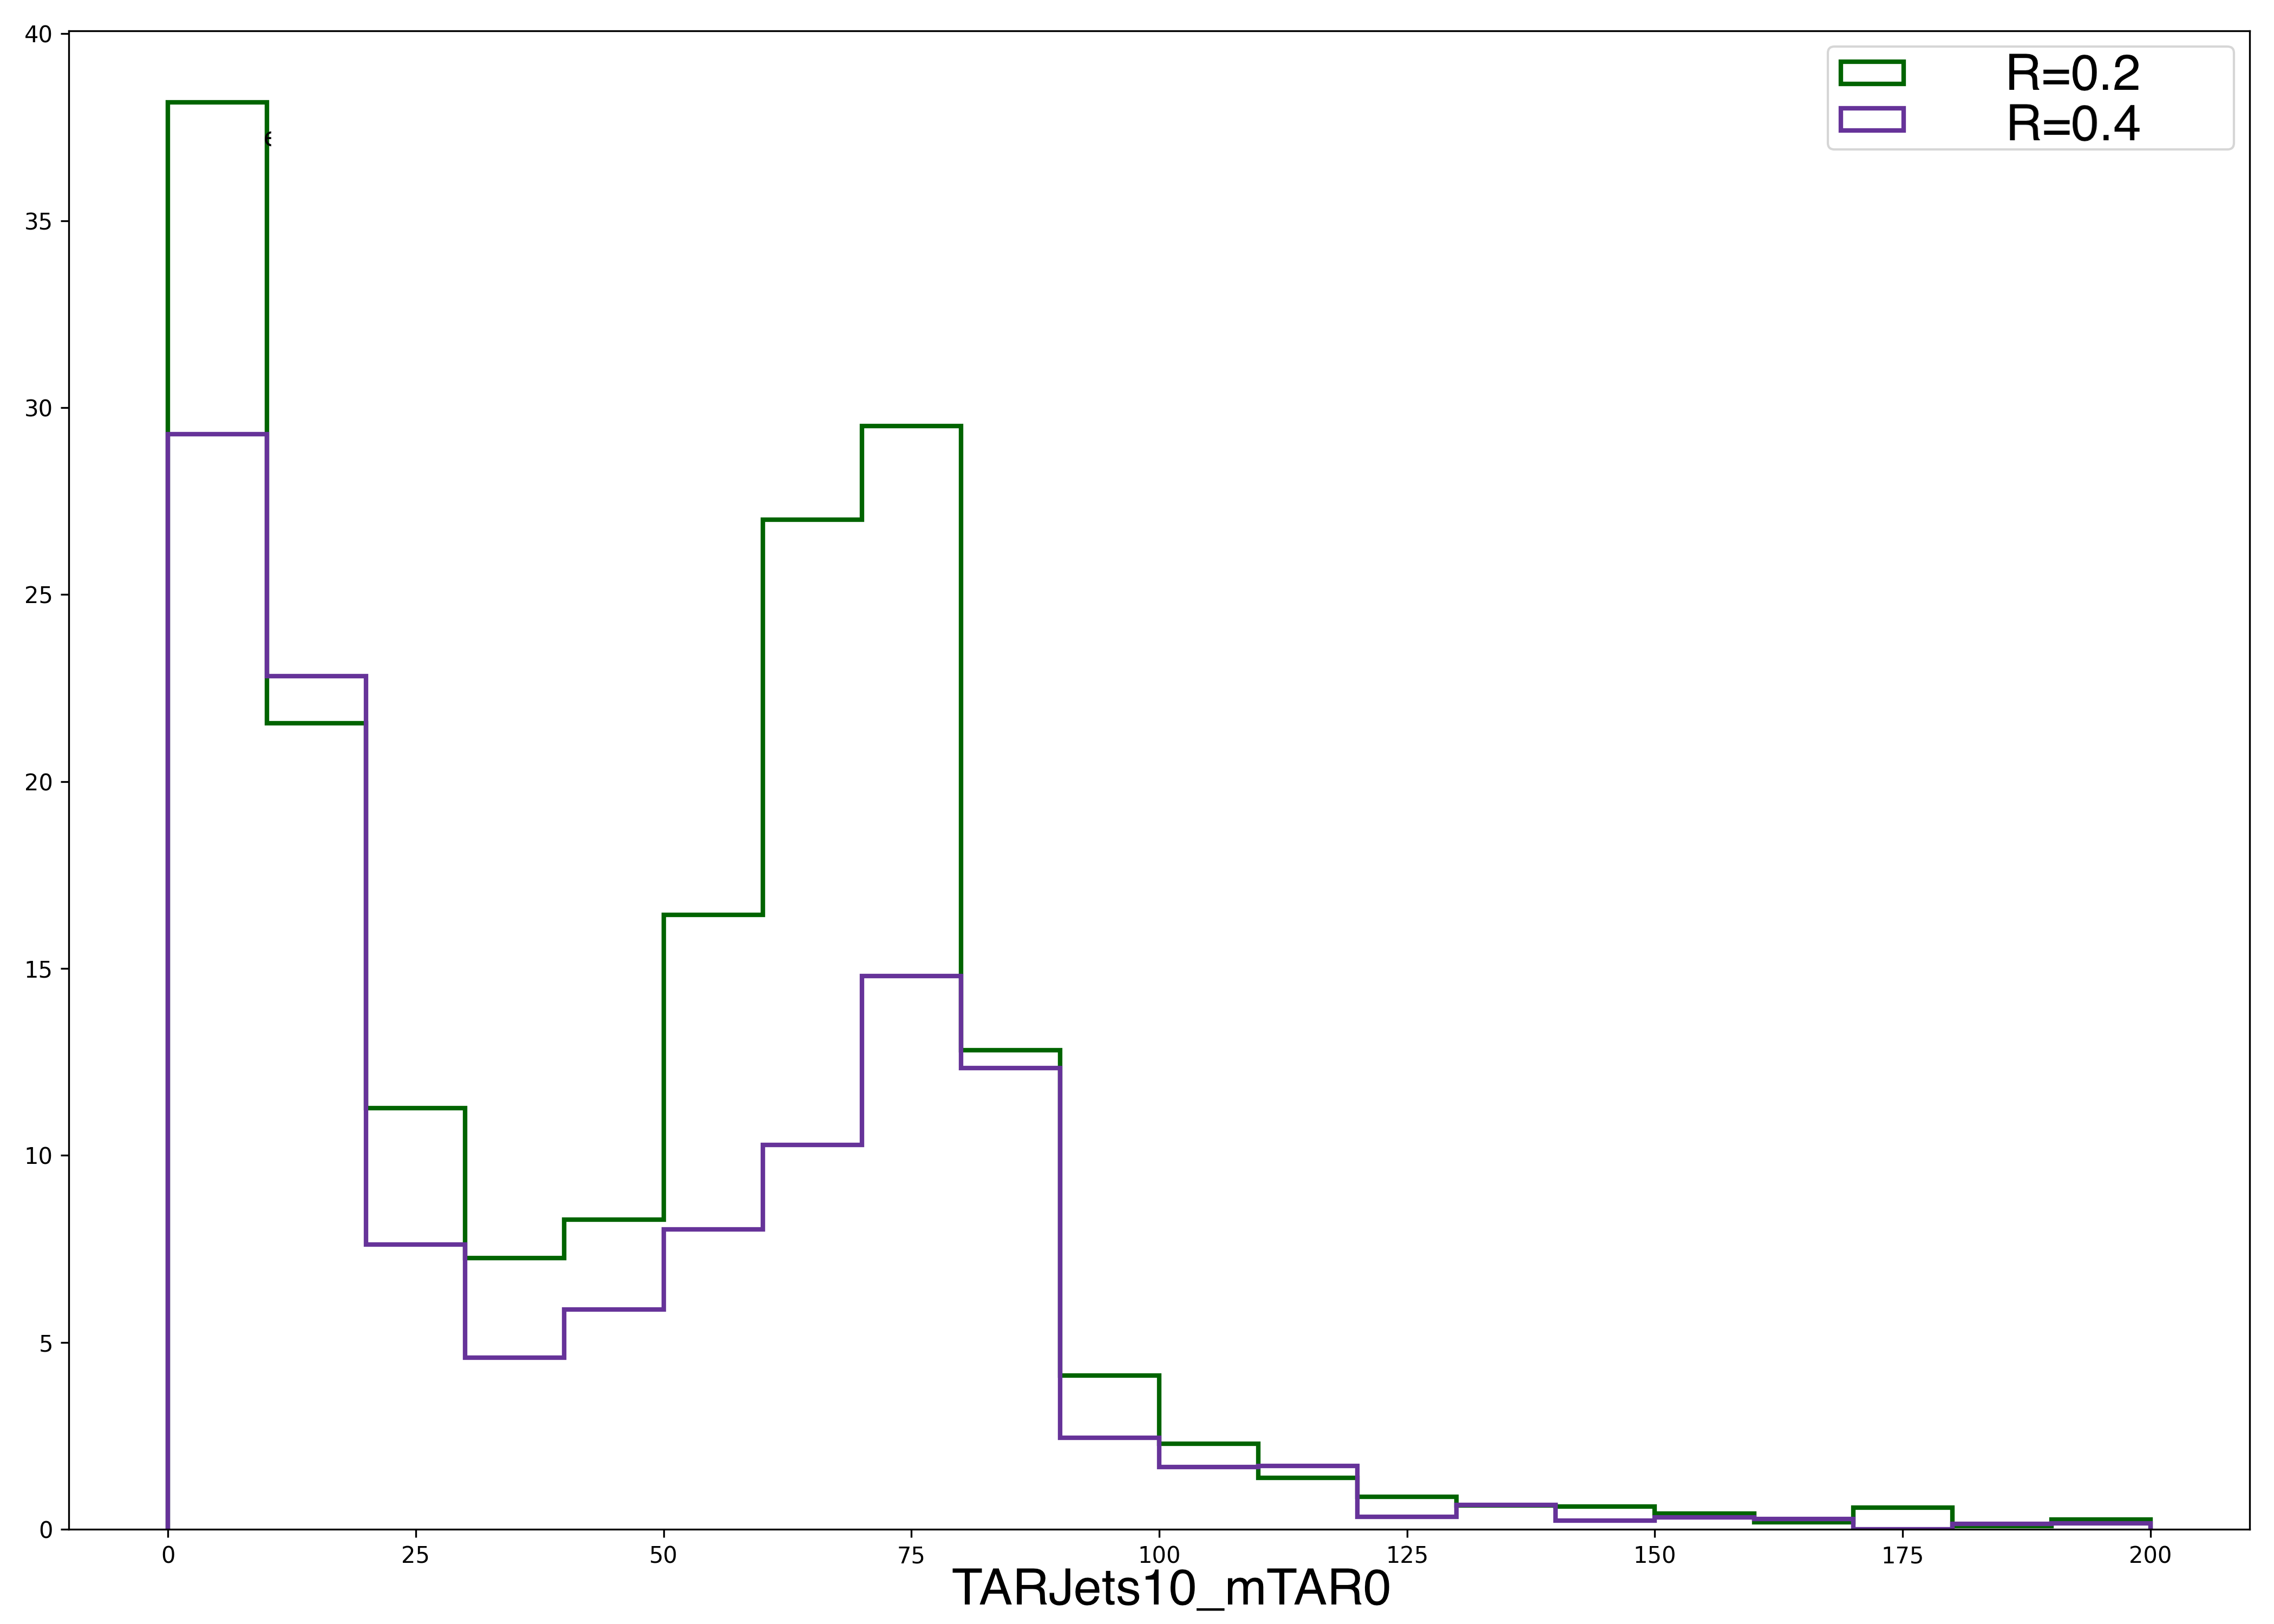
\includegraphics[width = 0.49\textwidth]{Figures/4/TAR/04_monoSww_semilep_zp1700_dm200_dh160.png}

     \caption{TAR jet mass distributions for two representative signal points, compared with constituent \akt $R=0.4$ vs.~\akt $R=0.2$ jets. Left: sample signal point at $(\ms, m_{Z^\prime})=(310, 500)$~GeV. Right: sample signal point at $(\ms, m_{Z^\prime})=(160, 1700)$~GeV.}
     \label{fig:R04_TAR_plots}
\end{figure}
\FloatBarrier
\subsection{Merged Signal Region Optimization}
\subsubsection{Asimov Significance}
We optimized the \merged signal region using the expected Asimov discovery significance $Z$ as the figure of merit  \cite{Asimov}. This is given by:
\begin{equation}
  Z = \left[ 2(s+b)\left(
    \ln\left[ \frac{(s+b)(b+\sigma_b^2)}{b^2 + (s+b)\sigma_b^2} \right]
    - \frac{b^2}{\sigma_b^2}\ln\left[ 1 + \frac{\sigma_b^2 s}{b(b+\sigma_b^2)} \right]
  \right) \right]^\frac{1}{2},
  \label{eq:asimov}
\end{equation}
where $b$ is the expected total number of background events, $s$ is the expected total number of signal events, and $\sigma_b$ is the uncertainty on the expected total number of background events. For a given set of selection criteria and signal point, this metric is calculated from the MC simulated data by applying the criteria, counting the number of remaining signal and background events, and computing their uncertainties, then calculating the significance. It provides a metric to assess the expected sensitivity of the signal region to the signal model.

\subsubsection{Optimization Approach}
In order to optimize the signal region selection, we employed a combination of an iterative visual approach and a computational approach. Visually, we studied the distributions of analysis variables, comparing signal and background distributions, to find areas of good discrimination where a cut placement might improve sensitivity. We then compiled a list of possible cuts in each of these areas of discrimination to form a basis for the computational optimization. To determine the optimal combination of these possible cuts, we created a script to test all possible combinations while computing the expected Asimov significance of each. When calculating significance during optimization, in addition to statistical uncertainty we applied a flat 20\% systematic uncertainty on the number of background events to more realistically reflect the expected total uncertainty. Different signal points in the \ms-\mZp plane have different kinematic properties, and cross-sections and therefore have different optimal selection. As a result, we selected the following four signal points at the edge of the search window for optimization:

\begin{itemize}
  \item (\ms, \mZp) = (310 GeV, 500 GeV),
  \item (\ms, \mZp) = (335 GeV, 1000 GeV),
  \item (\ms, \mZp) = (285 GeV, 1700 GeV),
  \item and (\ms, \mZp) = (210 GeV, 2100 GeV).
\end{itemize}

We then considered the cut combination with the highest mean expected Asimov significance over these four points to be optimal. In early iterations of optimization, the number of signal events selected using the optimal selection criteria was undesireably low. As a result, we implemented an additional requirement forcing the chosen criteria to maintain an expected yield of at least 15 signal events in the \merged signal region.

In order to avoid over-tuning the optimization on single events or statistical fluctuations, we spaced the lattice of possible cuts widely enough to allow several MC events to fall between each placement. Optimizing a selection in this manner also creates a systematic bias toward an under-prediction of background in the signal region, because a low expected background yield is considered desireable. To counter this bias, we used statistically-independent optimization and fitting data sets. We performed all optimization using a set of MC samples produced when using Sherpa 2.2.1 as a training set. A set of samples produced when using Sherpa 2.2.10 then provides a statistically-independent and more statistically rich data set which we used for validation and fit model testing. This means that the MC data used for fit model testing is isolated from the optimization of selection criteria.

\subsubsection{Optimization Variables}
We examined many analysis variables for potential sensitivity, and selected those having the best discrimination potential to be tested in the final optimization. Presented below is a list of variables tested and their meaning:

\begin{itemize}
  \item \textbf{\met} and \metsig: Missing transverse momentum; and the significance of its difference from a value of zero.
  \item \textbf{$p_T(\ell)$}: Transverse momentum of signal lepton.
  \item \textbf{\mtlepmet}: Transverse mass of lepton and \met system, given by
  \begin{equation}
  \mtlepmet = \sqrt{2 p_{\text{T},\ell} \met \left( 1 - \cos(\phi_\ell - \phi_{\met}) \right) }
  \end{equation}
  \item \textbf{\mTAR}: Mass of the \pT-leading TAR jet calculated from the rescaled matched tracks.
  \item \textbf{\ptTAR}: Transverse momentum of the leading TAR jet.
  \item \textbf{\DtwoTAR}: Energy correlation function of the TAR jet, which helps to identify two-pronged jet substructure \cite{DTwo}.
  \item \textbf{TAR Jet $\tau_{42}^{WTA}$ and $\tau_{21}^{WTA}$}: ``$n$-Subjettiness" ratios of the leading TAR jet, to identify two-pronged substructure \cite{Tau42}.
\end{itemize}

In addition, we considered a two-dimensional cut above or below a line with variable slope and intetcept in the \met-$p_T(\ell)$ plane during optimization.

\subsubsection{Optimized Selection}

We found the maximum mean expected significance across the four selected signal points to be achieved using the selection shown in Table \ref{tab:mergedselection_reopt}.

\begin{table}[t]
  \centering
  \begin{tabular}{c|c|c}
    \toprule
    \textbf{variable}  &  \textbf{requirement} &  \textbf{reason}  \\
    \midrule
    \NTAR  &  $>0$ & \Wcand reconstruction \\
    \mtlepmet  &  $>220\,\GeV$ & $W$+jets background reduction\\
    \mTAR &  $[68,89]\,\GeV$ & \Wcand reconstruction \\
    \metsig  &  $>16$ & Select for high \met \\
    \dRTARl &  $<1.2$ & Select for boosted \Wcand+$\ell\nu$ system \\
    \DtwoTAR  &  $<1.1$ & 2-pronged $W\rightarrow qq$ reconstruction \\
    \bottomrule
  \end{tabular}
  \caption{Optimized selection criteria for the \merged category signal region.}
  \label{tab:mergedselection_reopt}
\end{table}

In order to validate this choice of selection criteria, we produced ``$N-1$" plots which show the distribution of a variable with all but the cut on that variable applied. We also calculated the expected Asimov significance of placing a cut at each bin edge in the ``$N-1$" histogram. We then compared the optimized cut placement with the cut placement showing maximal expected significance in the plot. These plots were produced using the testing and validation data ($W$+jets and $Z$+jets samples produced in Sherpa 2.2.10), and are shown in Figure \ref{fig:SRN1}. They show that the cuts optimized using Sherpa 2.2.1 samples are still placed at optimal or near-optimal locations using the final samples, and therefore validate the choice of selection criteria. To produce these plots, a single event with a large negative weight was removed from the background MC, as its weight overwhelmed the shape of the background distributions and produced sharp spikes in estimated significance. A secondary set of N-1 plots with this event included are shown in Appendix section \ref{section:N1_backup}

\begin{figure}[htbp]
  \centering

     \begin{subfigure}{0.49\textwidth}
     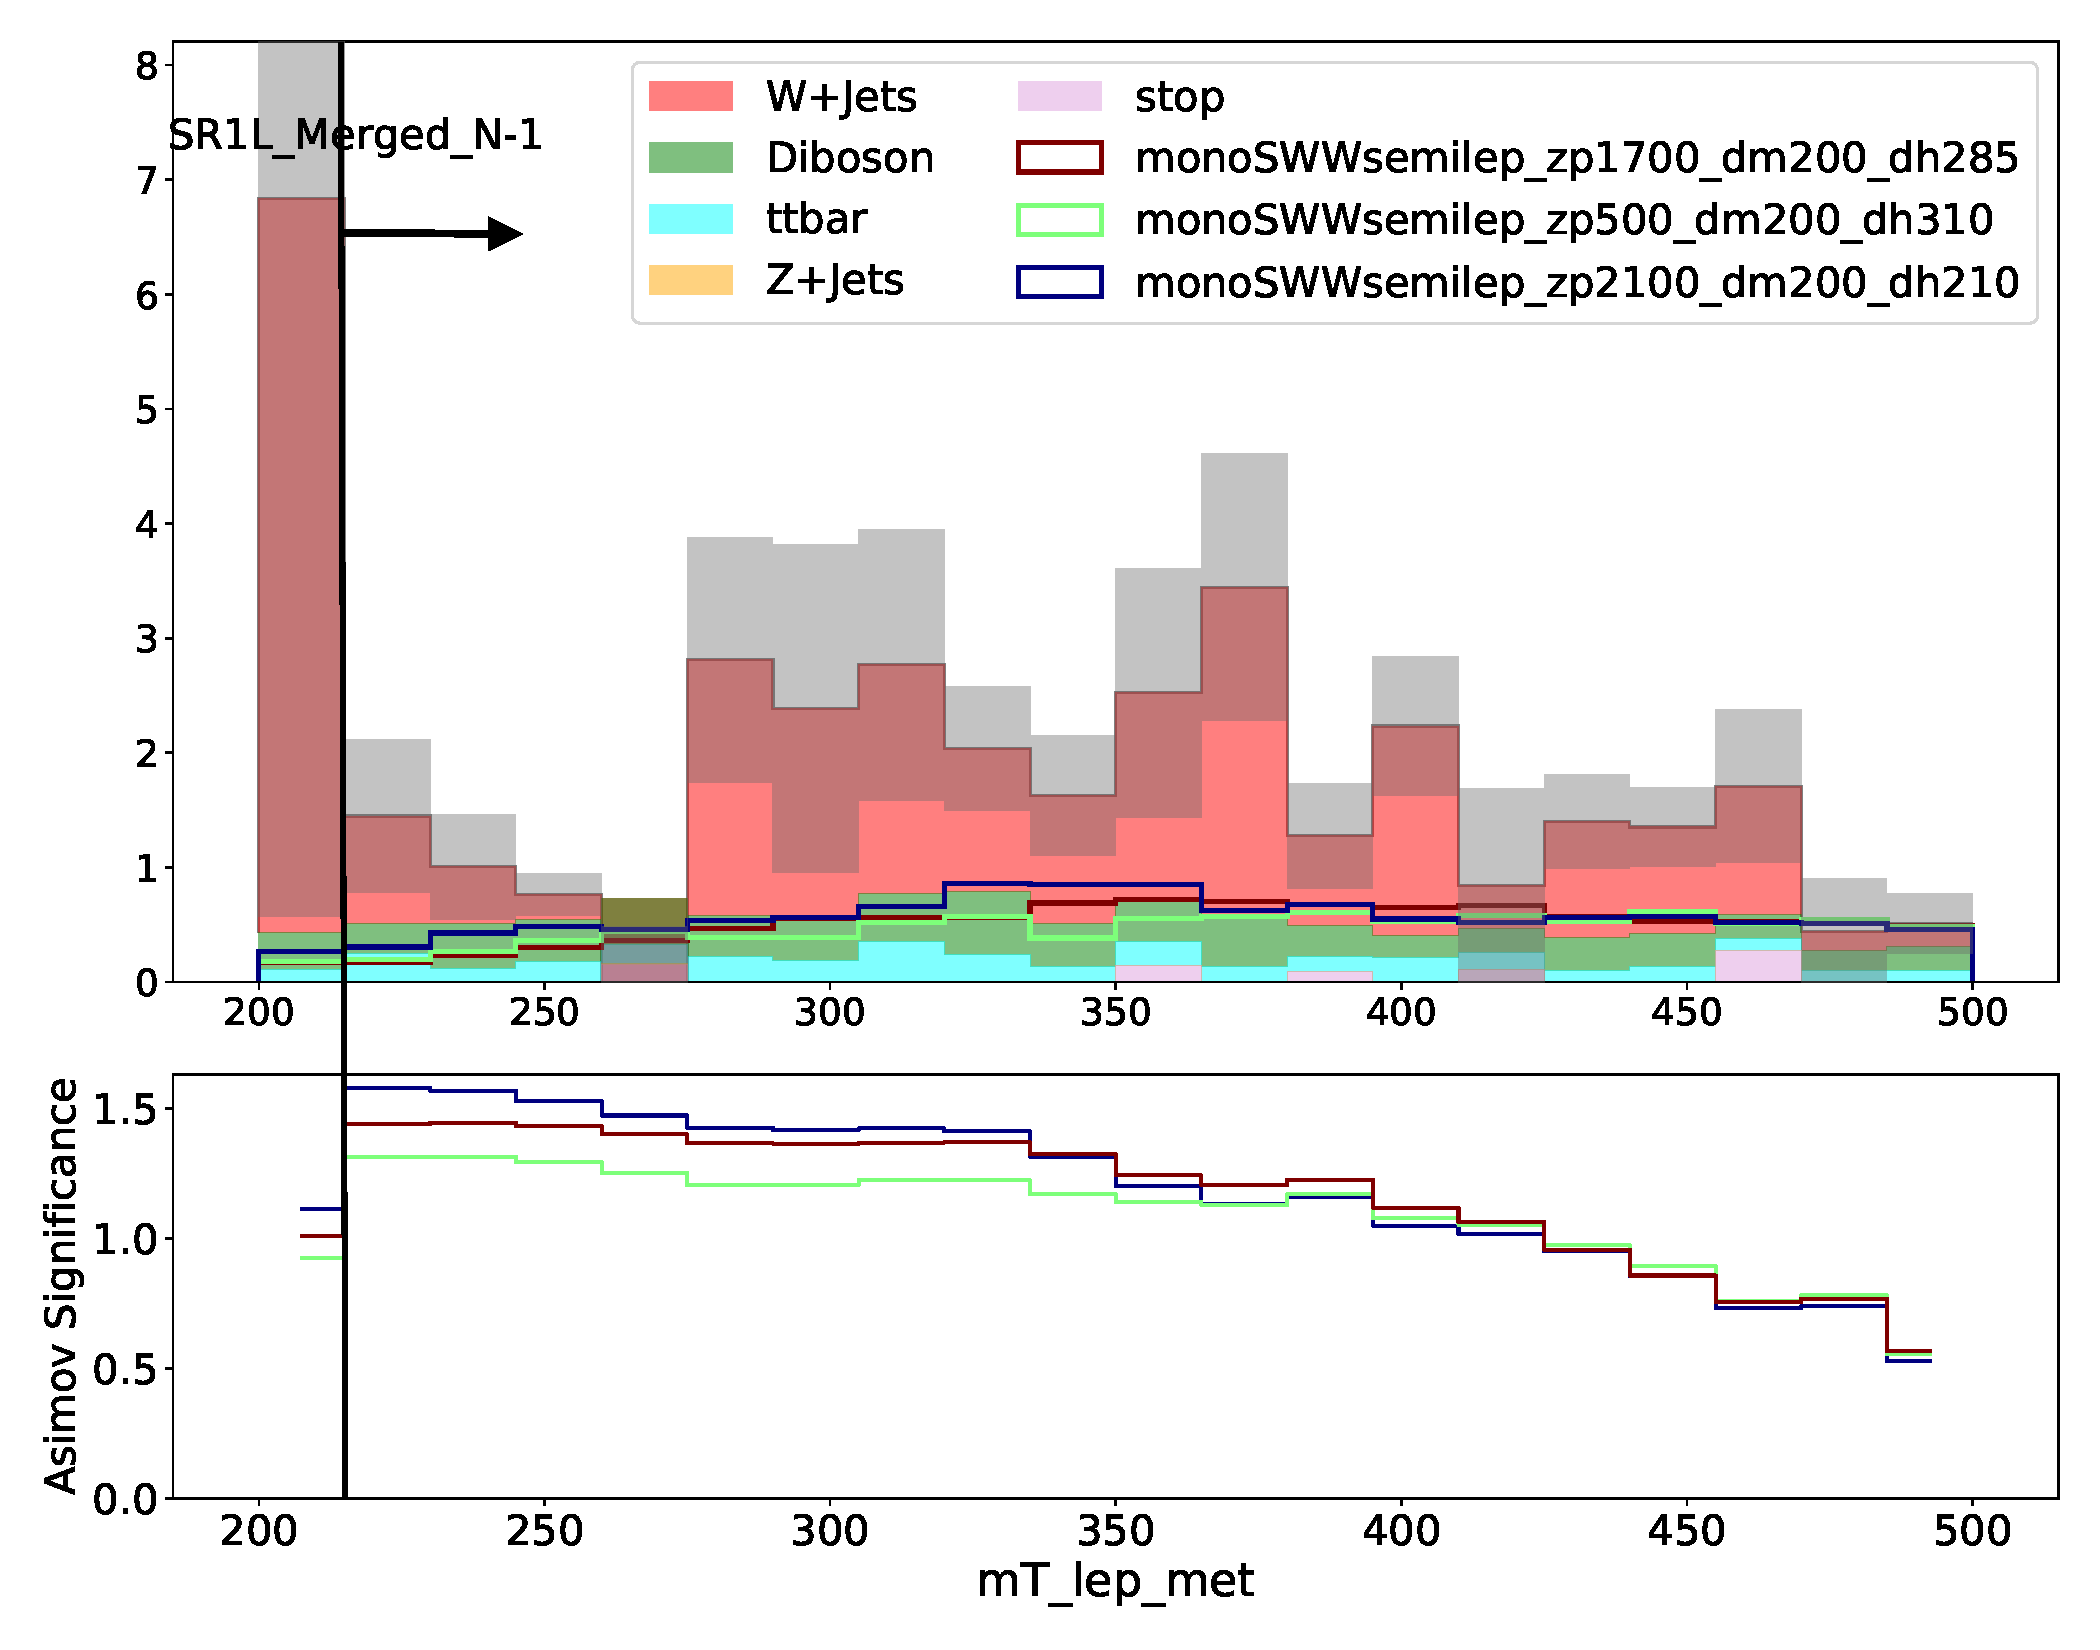
\includegraphics[width = 0.98\textwidth]{Figures/4/N1m/mT_lep_met.pdf}
     \caption{\mtlepmet}
     \end{subfigure}
     \begin{subfigure}{0.49\textwidth}
     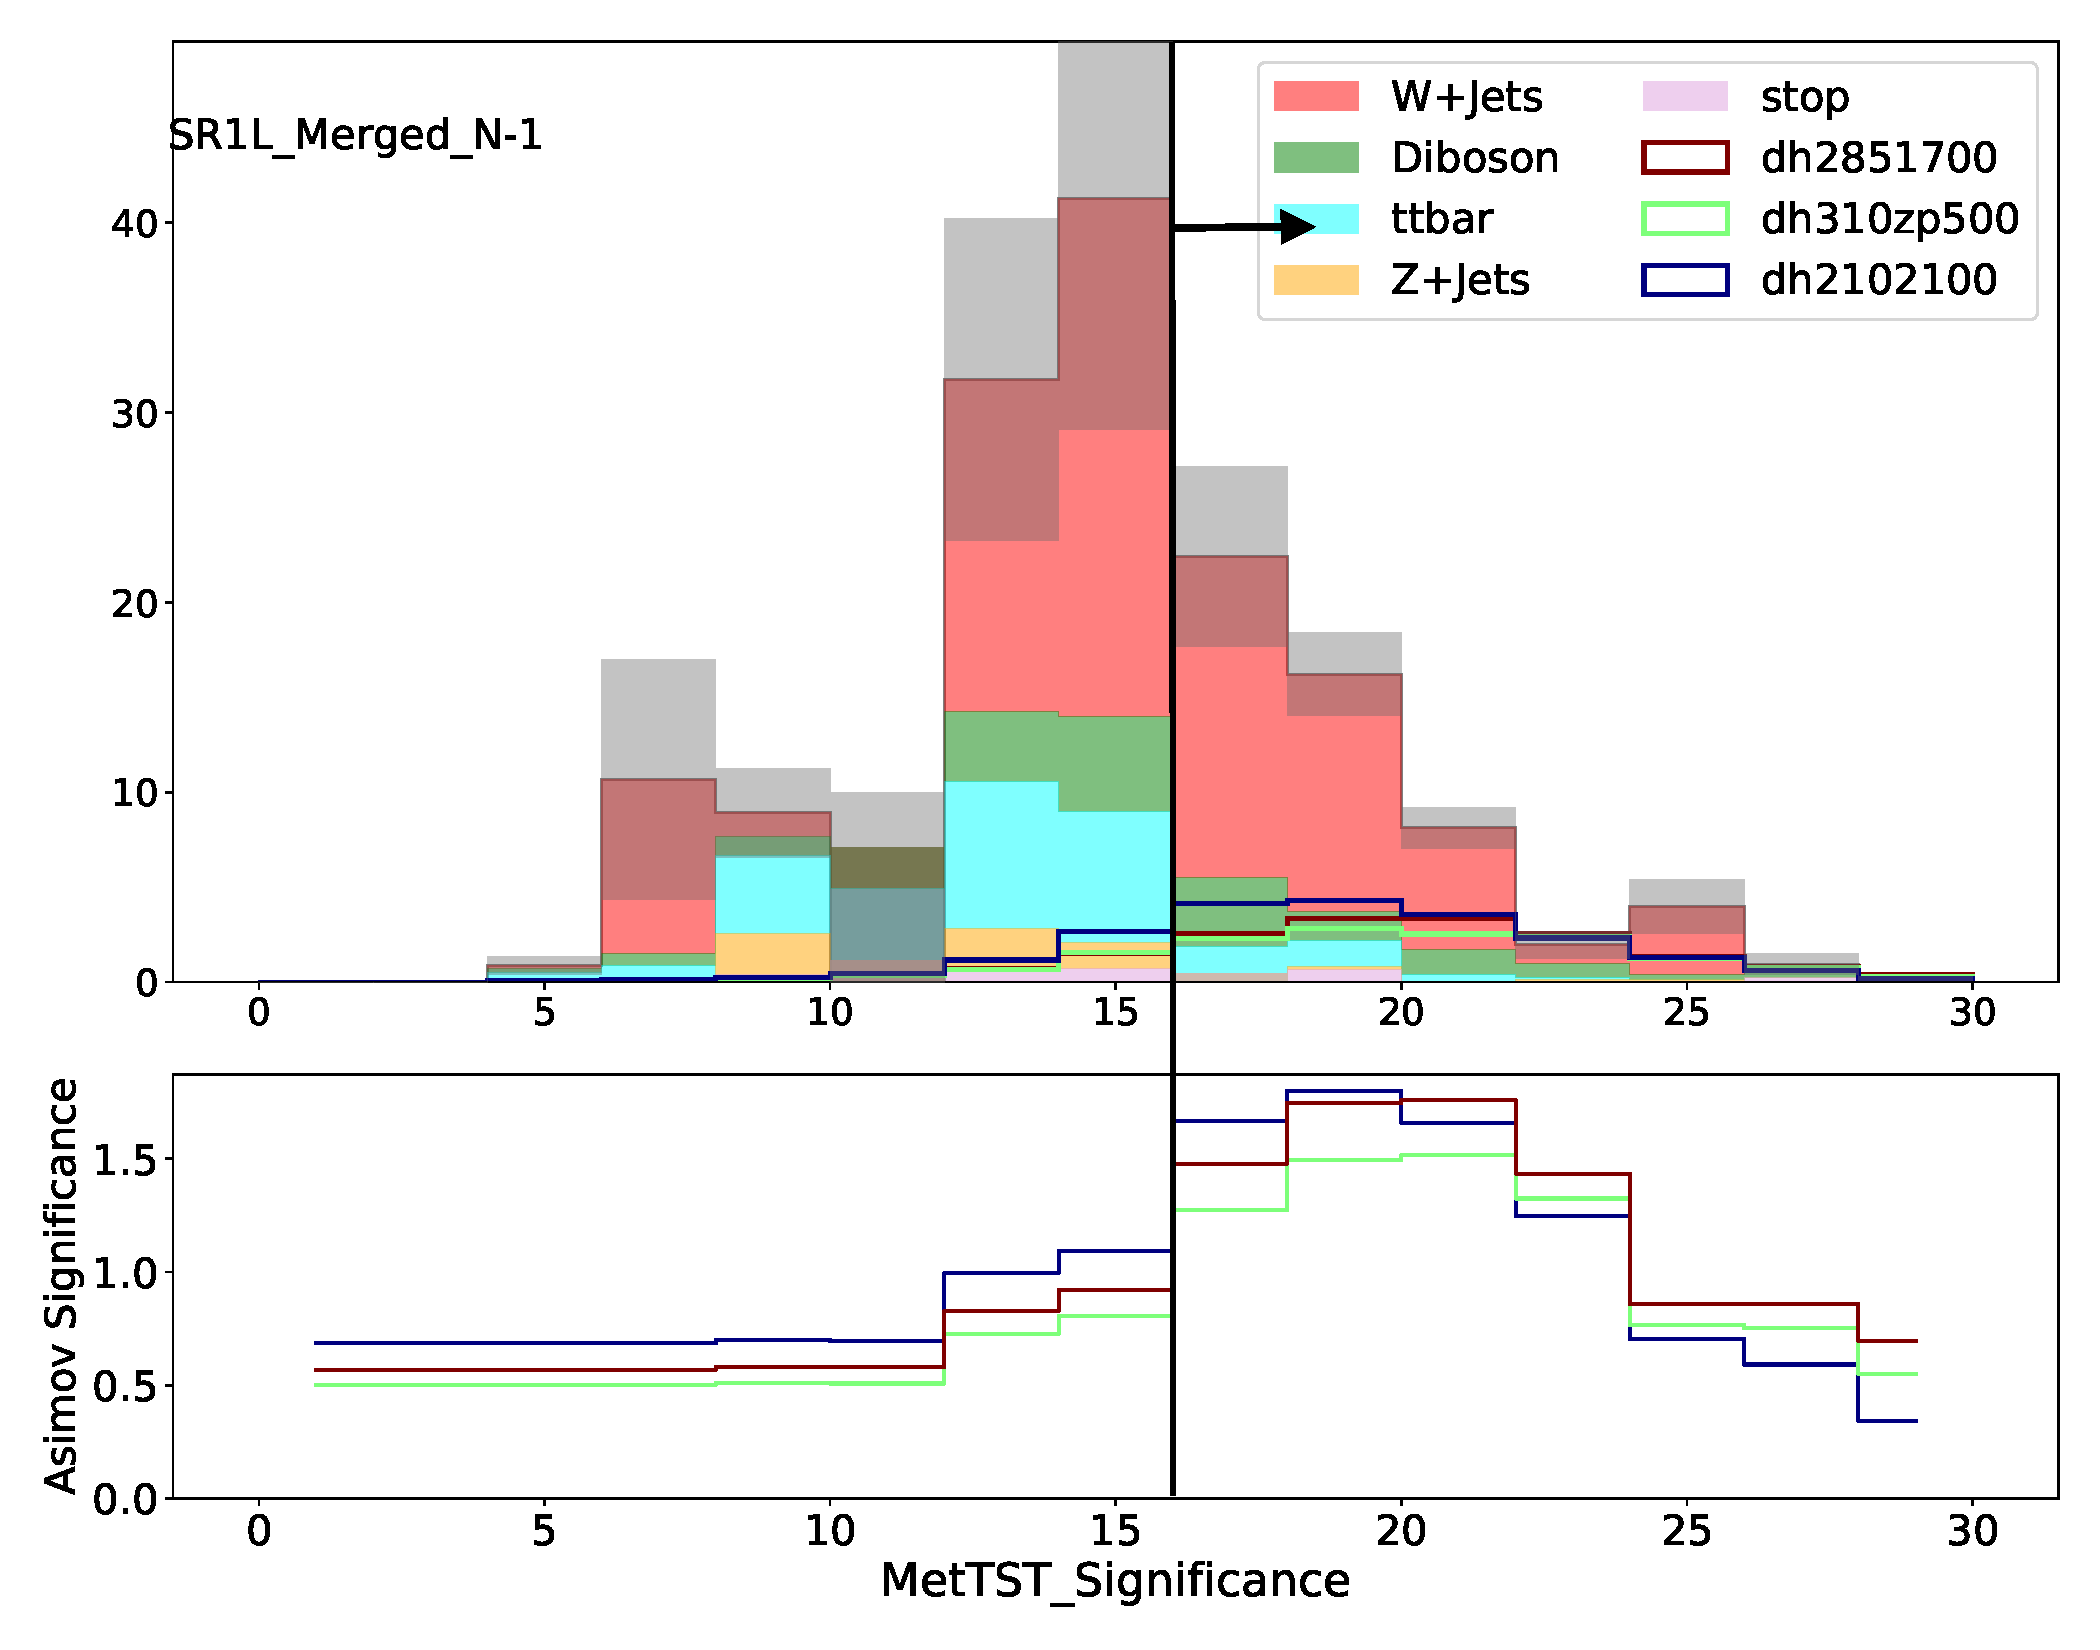
\includegraphics[width = 0.98\textwidth]{Figures/4/N1m/MetTST_Significance.pdf}
     \caption{\metsig}
     \end{subfigure}
     \begin{subfigure}{0.49\textwidth}
     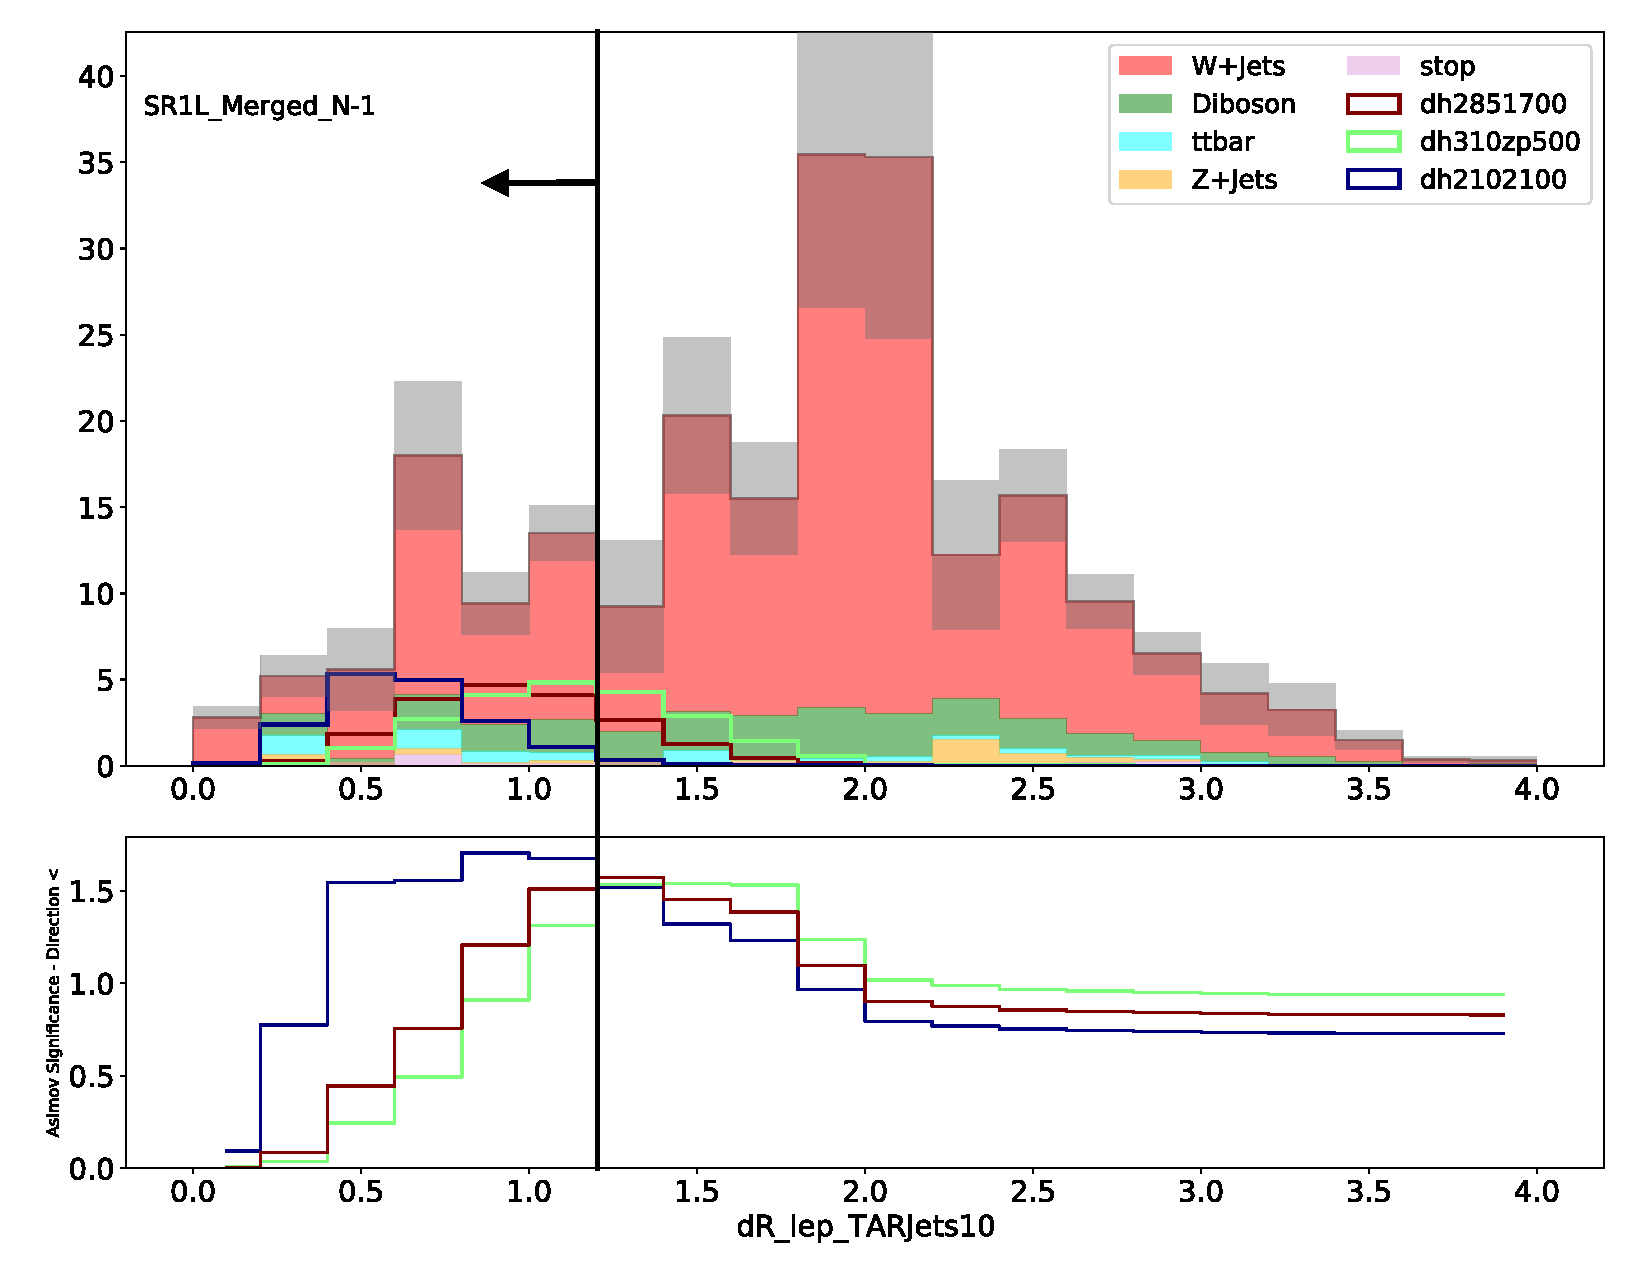
\includegraphics[width = 0.98\textwidth]{Figures/4/N1m/dR_lep_TARJets10.pdf}
     \caption{\drTARl}
     \end{subfigure}
     \begin{subfigure}{0.49\textwidth}
     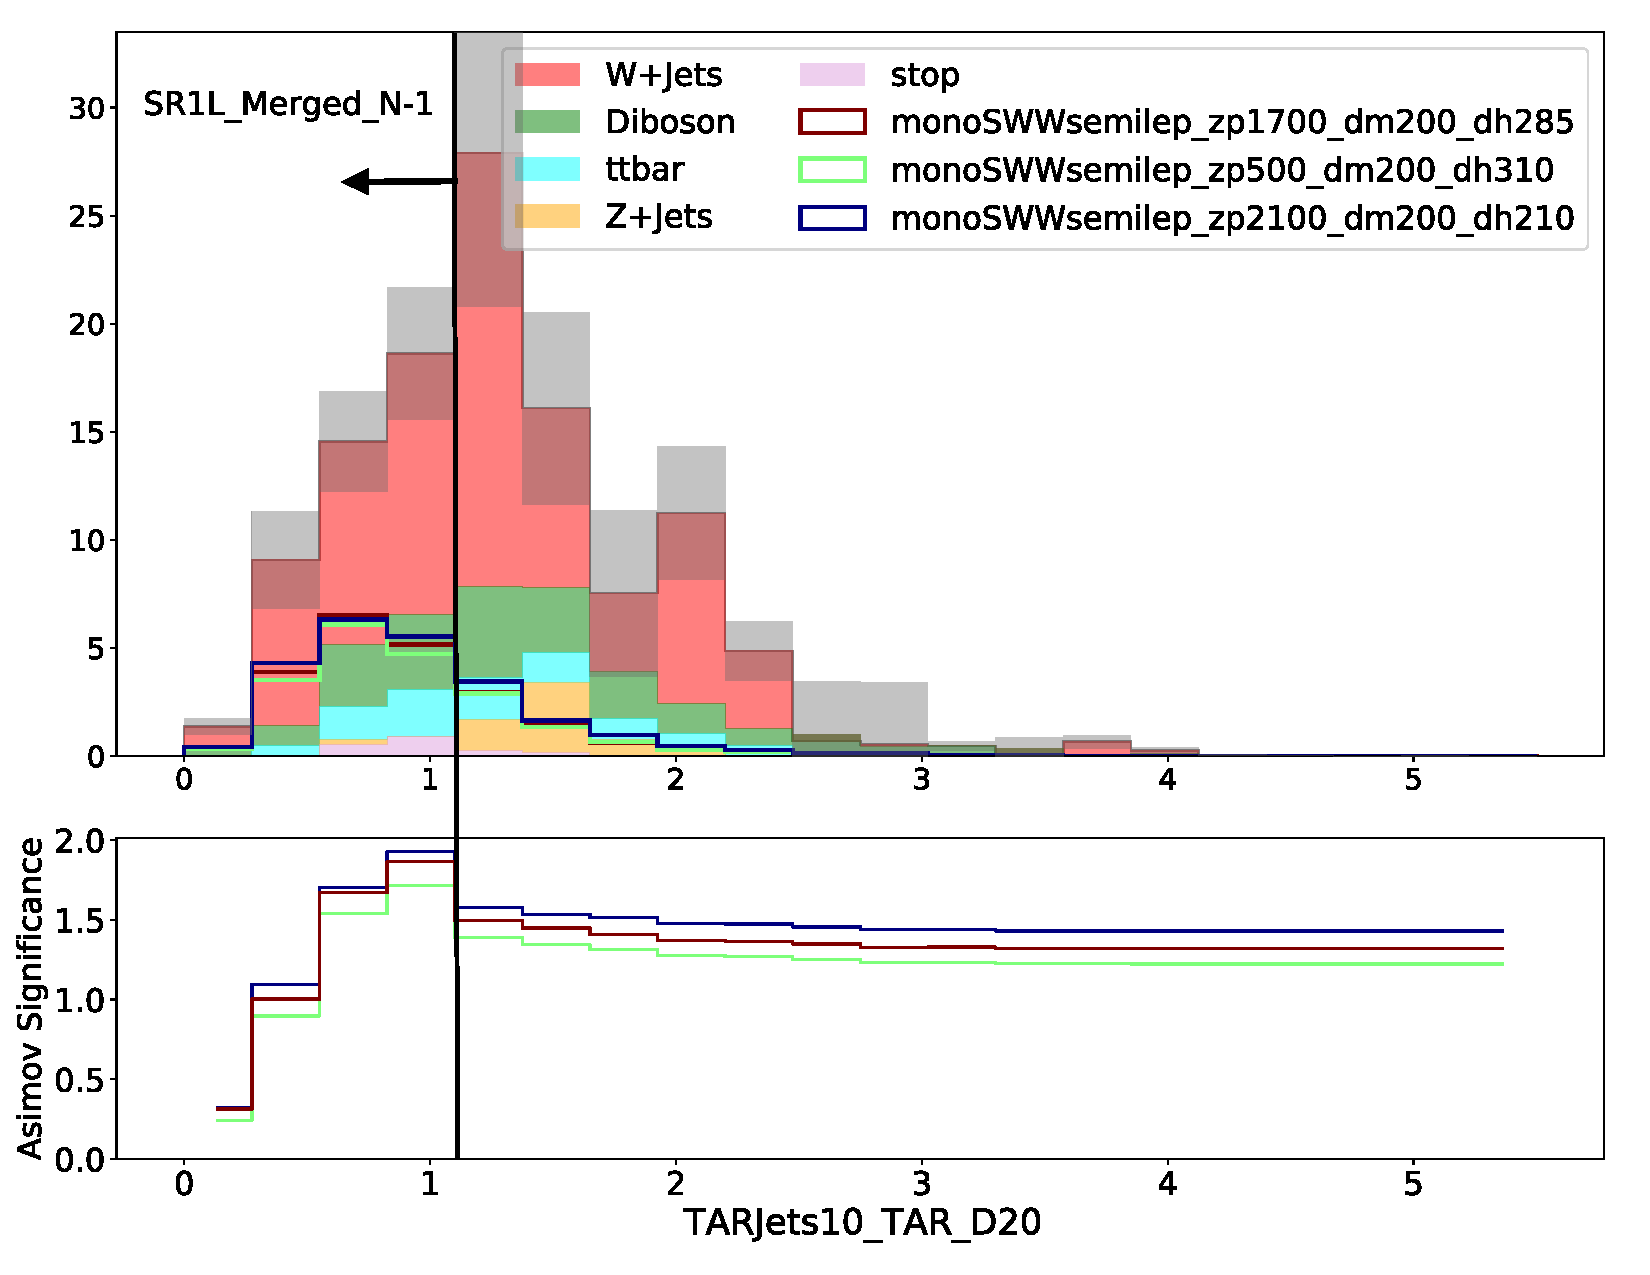
\includegraphics[width = 0.98\textwidth]{Figures/4/N1m/TARJets10_TAR_D20.pdf}
     \caption{\DtwoTAR}
     \end{subfigure}
     \begin{subfigure}{0.49\textwidth}
     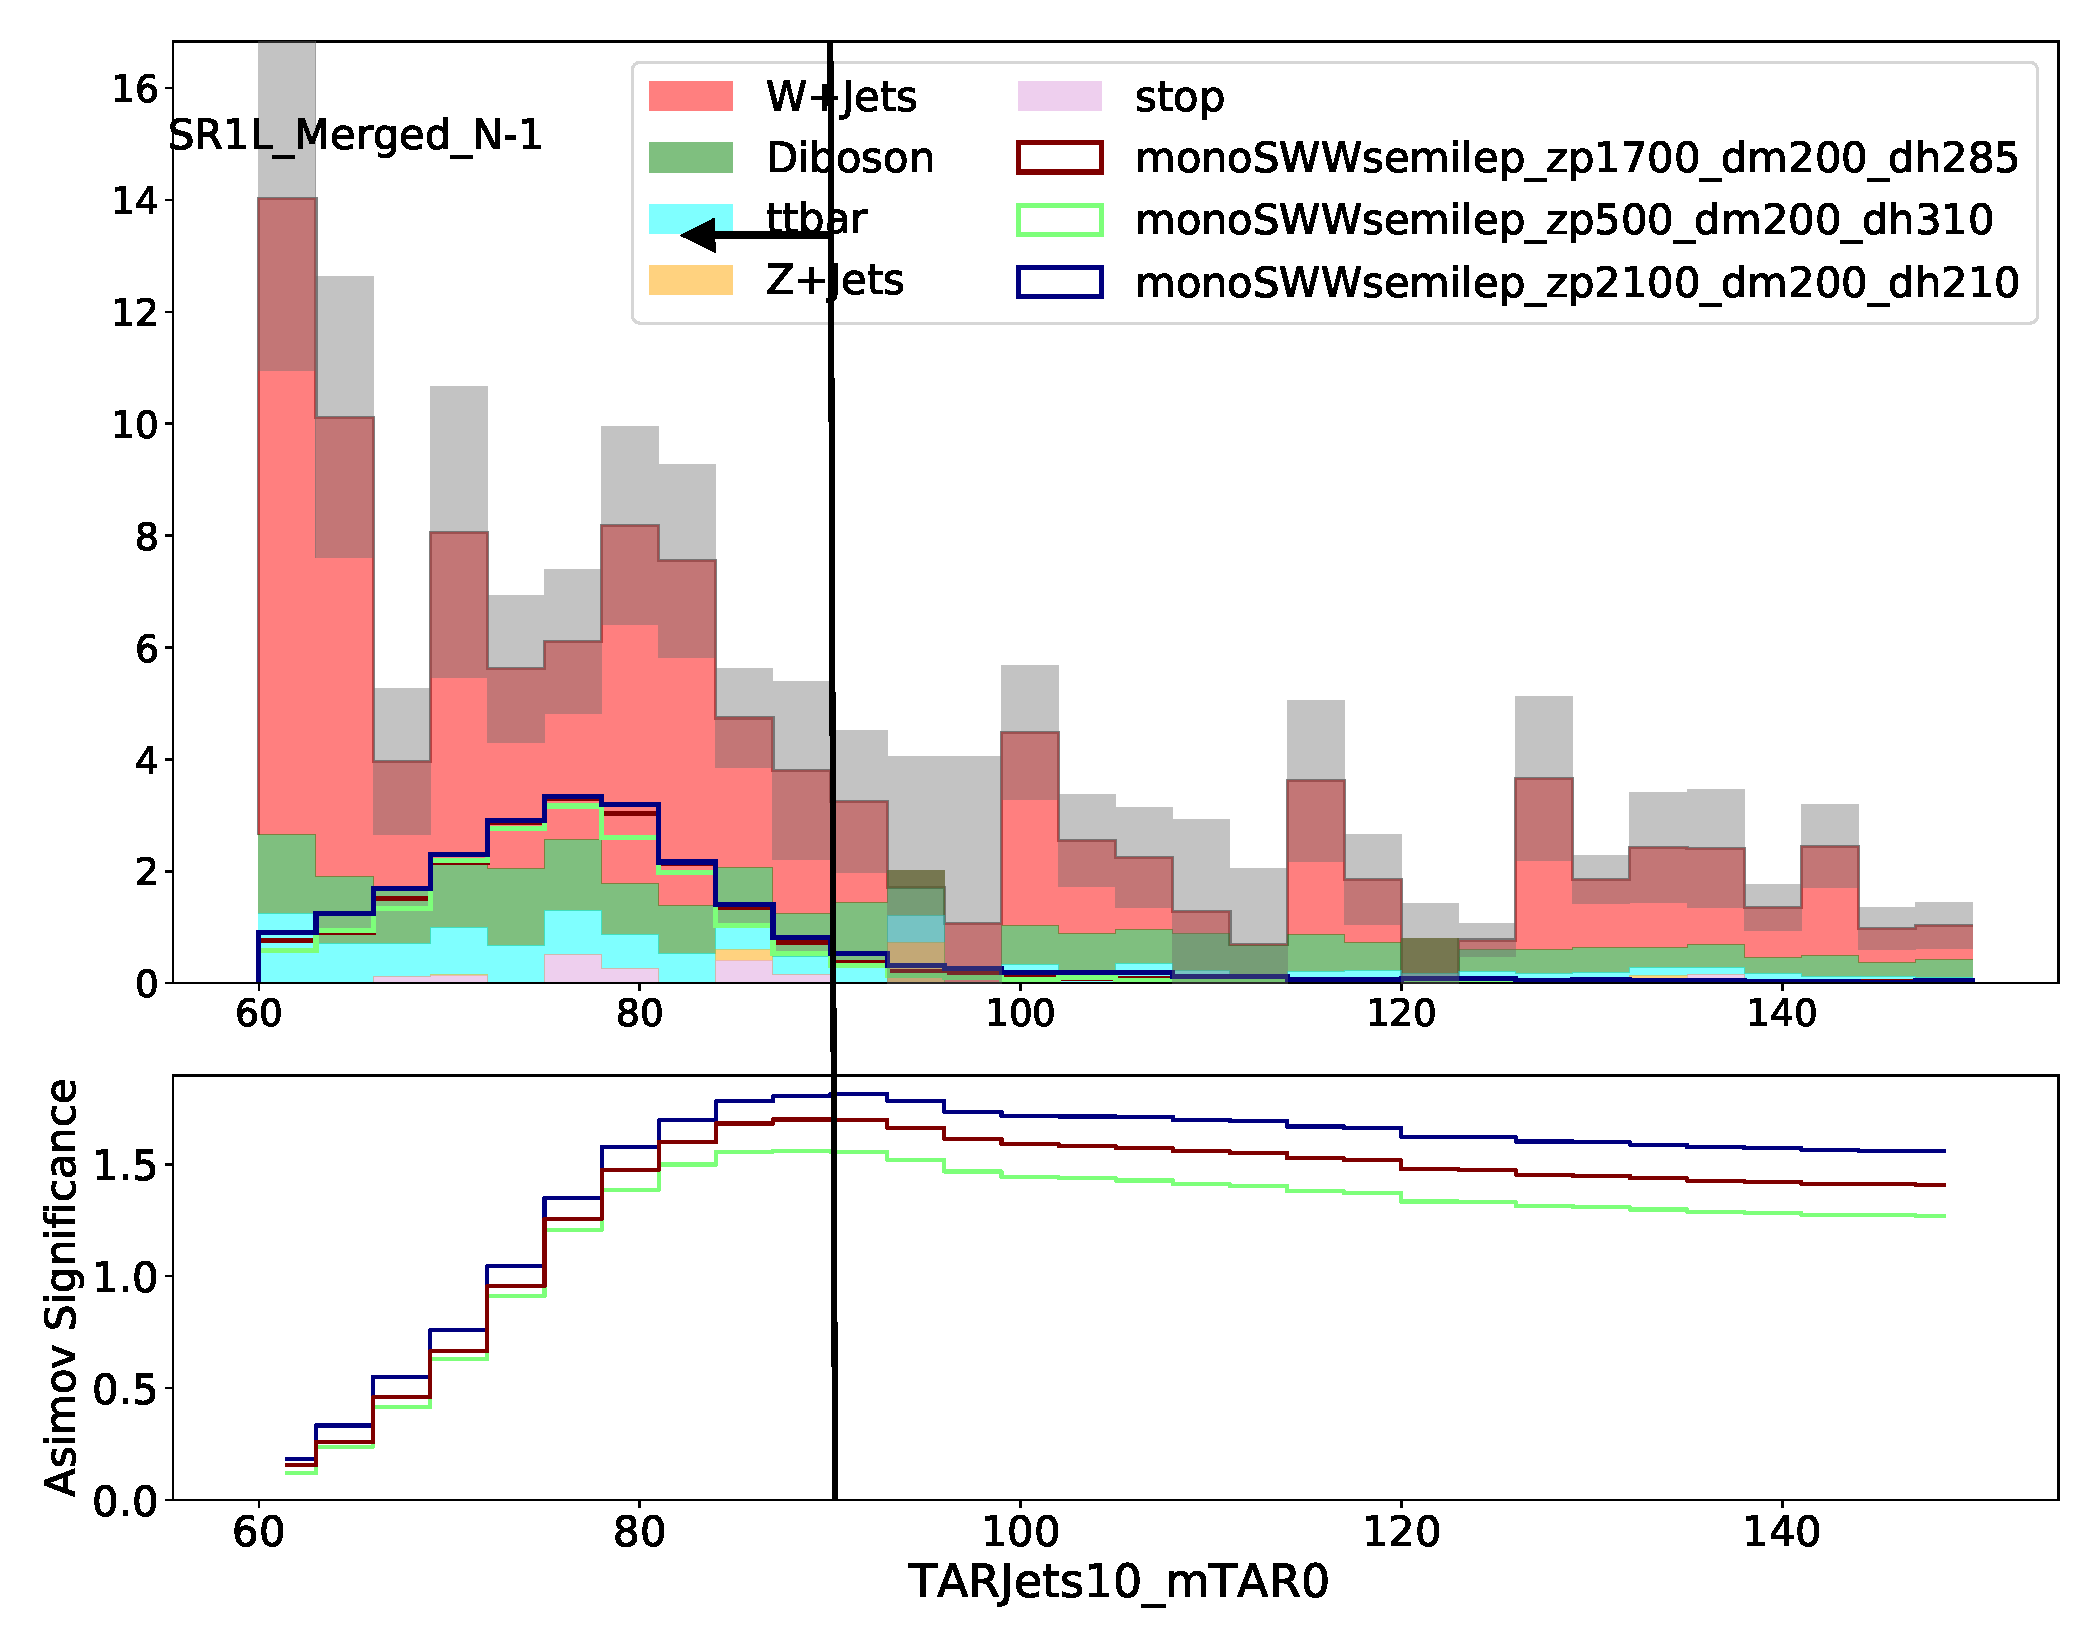
\includegraphics[width = 0.98\textwidth]{Figures/4/N1m/TARJets10_mTAR0.pdf}
     \caption{\mTAR}
     \end{subfigure}
     \begin{subfigure}{0.49\textwidth}
     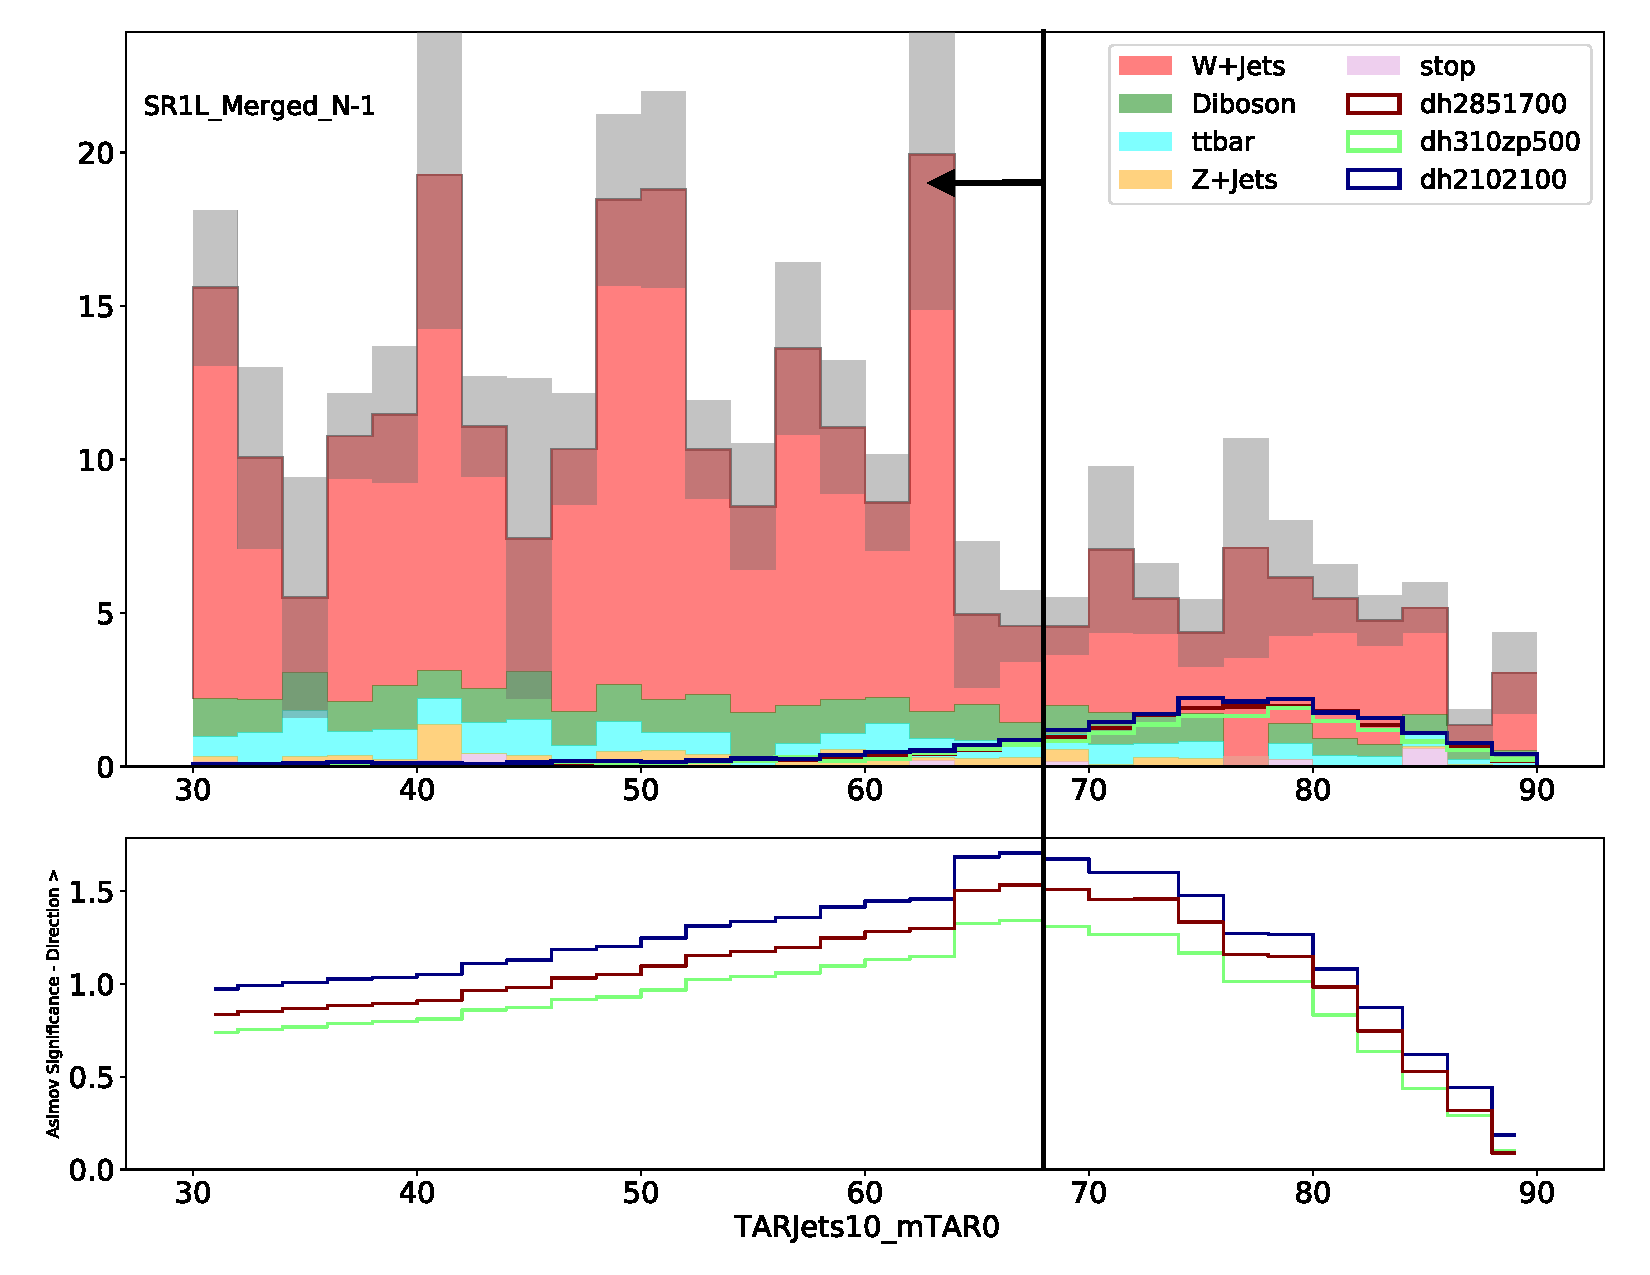
\includegraphics[width = 0.98\textwidth]{Figures/4/N1m/TARJets10_mTAR02.pdf}
     \caption{\mTAR}
     \end{subfigure}

     \caption{``$N-1$" plots in the \merged signal region showing the distribution of variables with all cuts applied except that of the variable shown. Grey bands represent MC statistical uncertainty on each bin.}
     \label{fig:SRN1}
  \end{figure}
\FloatBarrier

\section{Resolved Signal Region}
Due to the highly boosted nature of most signal events, the hadronic $W$ decay products are often best resconstructed as an $R=1.0$ TAR jet. To capture events for which this is not the best reconstruction we define our \resolved signal region. Being a secondary region, the \resolved signal region is considerably less sensitive to the signal model than the \merged signal region, but does provide some enhancement especially at low $s$ mass where the least boost is experienced. The \resolved signal region selection criteria are listed in Table \ref{tab:Resolved_SR_Cuts}.

\begin{table}[htbp]
\caption{Overview of \resolved SR cuts.}
\label{tab:Resolved_SR_Cuts}
\centering
  \begin{tabular}{c | c  }
  \toprule
 \textbf{cut} &  \textbf{reason} \\
  \midrule
Fails \merged analysis region selections & Recycling strategy \\
  \Njets $\geq 2$ & \Wcand reconstruction \\
 $\Wcandm \in [65,95]~\GeV$ & \Wcand reconstruction \\
 $ \Wcandpt > 150~\GeV$ & $W$+jets Background Reduction \\
  $\mtlepmet > 200~\GeV$ & $W$+jets Background Reduction \\
  $\met  > 250$ GeV & Select for high \met \\
  $\metsig  > 16$ & Select for good \met \\
  $\drWl  < 1.4$ & Select for boosted \Wcand+$\ell\nu$ system \\
  %Lepton \pt & $<\met-70~\GeV$ \\
  \bottomrule
  \end{tabular}
\end{table}

\section{\ttbar Control Regions}
A control region is used to help constrain one or more sources of background in an analysis. It is designed as a region that covers a similar but non-overlapping area of phase space to the signal region, and is expected to contain many fewer signal events. As a result, the number of observed ATLAS data and MC-predicted SM events should match very closely. Any difference provides information about how MC predictions differ from data observations and is used derive a normalization factor to constrain the SM background predictions of MC in the signal region, and provide a more accurate projection.

To design an effective control region, we attempted to satisfy four important criteria:
\begin{itemize}
  \item \textbf{Non-overlap with the signal region:} This ensures that the sample used to constrain the signal region background is statistically-independent from the signal region.
  \item \textbf{High \ttbar purity:} This selects for the background of interest in the control region to better individually constrain that background.
  \item \textbf{Low signal contamination:} This ensures that the comparison of ATLAS data and MC in this region is not affected by the signal model and effectively constrains only the SM background.
  \item \textbf{Similar kinematics to SR:} This ensures that a similar region of phase space is being studied in the control and signal regions, so that the normalization factors derived apply well to both regions.
\end{itemize}

The fact that \ttbar is one of the sub-dominant backgrounds in both signal regions motivated me to create one such control region for each signal region. As a consequence of top quarks decaying primarily to a $W$ boson and $b$-quark, the principal cut excluding \ttbar events from the signal regions is the veto of any events containing a $b$-tagged \akt $R=0.4$ jet. We therefore chose to try defining a similar but non-overlapping region rich in \ttbar events by simply reversing this cut and also requiring at least 1 $b$-tagged jet. We found this proposed region to be too rich in expected signal events, however, with signal yields as high as 10\% of background yields in the \merged region.

To improve this, we further extended the $b$-jet cut to require 2 or more $b$-jets in the control region. This change sufficiently reduced signal contamination, but in the \merged control region it had the additional consequence of substantially reducing the number of events in the region, thereby reducing its statistical power.  In response we also loosened the \metsig cut in the \merged \ttbar control region to \metsig > 12, considerably improving the \ttbar yield. To inform this choice, we used figure \ref{fig:ttbar_metsig_placement}, which shows the number of weighted \ttbar events expected within the \merged control region for a given \metsig cut.

\begin{figure}[htbp]
    \centering
       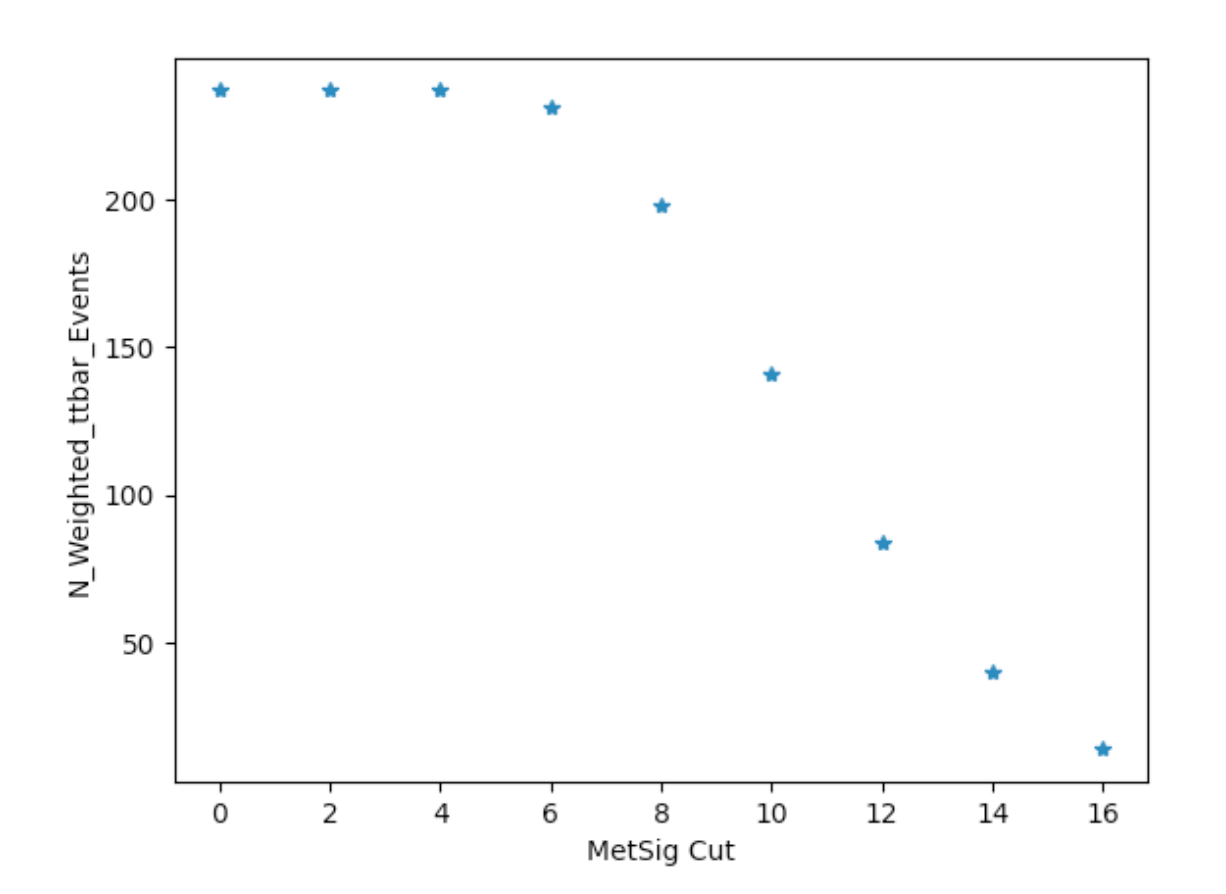
\includegraphics[width = 0.80\textwidth]{Figures/4/ttbarCR/ttbar_metsig_placement.png}
       \caption{\ttbar yield in the \merged \ttbar control region for various \met significance cut placements.}
       \label{fig:ttbar_metsig_placement}
\end{figure}

\begin{table}[t]
 \centering
\begin{tabular}{l|l|l}
\toprule
\textbf{Region} & \ensuremath{N (b\text{-jets})} Cut & \metsig Cut \tabularnewline
\midrule
\textbf{Merged SR} & \ensuremath{N (b\text{-jets})} = 0 & $\metsig > 16$\tabularnewline
\midrule
\textbf{Resolved SR} & \ensuremath{N (b\text{-jets})} = 0 & $\metsig > 16$\tabularnewline
\midrule
\textbf{Merged CRtt} & \ensuremath{N (b\text{-jets})} > 1 & $\metsig > 12$\tabularnewline
\midrule
\textbf{Resolved CRtt} & \ensuremath{N (b\text{-jets})} > 1 & $\metsig > 16$\tabularnewline
\bottomrule
\end{tabular}
\caption{\label{tab:ttbar_CR} Summary of differences in selections on \ensuremath{N (b\text{-jets})} and \metsig between signal regions and \ttbar control regions.}
\end{table}

Table \ref{tab:ttbar_CR} summarizes the differences in selection criteria between the \merged and \resolved signal and \ttbar control regions. Figures \ref{fig:Data_MC_CRbV_merged} and \ref{fig:Data_MC_CRbV_resolved} in Appendix section \ref{section:datamc} show comparisons of the distributions of MC and ATLAS data in the \ttbar control regions. These demonstrate a slight over-prediction of background from MC in the \merged region, which is used during fitting to constrain the \ttbar background in the signal region. The difference between data and MC distributions does not show a strong correlation with any of the analysis variables. To ensure that the kinematic qualities of the signal and control regions are sufficiently similar to provide a good constraint, Figures \ref{fig:CRSR_merged} and \ref{fig:CRSR_resolved} in Appendix section \ref{section:CRSR} show comparisons of distributions of key kinematic variables between the \merged and \resolved control and signal regions.

\FloatBarrier
\section{\wjets Control Region}
\FloatBarrier
This analysis employs an additional pair of control regions in order to constrain the dominant \wjets background in the signal regions. The signal regions occupy a realm of phase space very high in \mtlepmet, and we sought to better constrain the background prediction in the tail of this distribution. To achieve this we defined control regions by reversing the \drTARl and \drWl cuts in the \merged and \resolved signal regions. This reverses the direction of the neutrino and charged lepton in the leptonic $W$ decay without substantially altering the remaining kinematics of the event, keeping the region high in \mtlepmet. In the \merged \wjets control region we again reduced the \metsig cut to \metsig > 12 in order to improve statistical power. We then further extended the \drTARl requirement to $\drTARl > 1.8$ in the merged control region to reduce signal contamination.
Table \ref{tab:Wjets_CR} summarizes the differences in selection criteria between the \merged and \resolved signal and \wjets control regions.
\begin{table}[h]
 \centering
\begin{tabular}{l|l|l}
\toprule
\textbf{Region} & $\Delta R$ Cut & \metsig Cut \tabularnewline
\midrule
\textbf{Merged SR} & $\drTARl < 1.2$ & $\metsig > 16$\tabularnewline
\midrule
\textbf{Resolved SR} & $\drWl < 1.4$ & $\metsig > 16$\tabularnewline
\midrule
\textbf{Merged CRW} & $\drTARl > 1.8$ & $\metsig > 12$\tabularnewline
\midrule
\textbf{Resolved CRW} & $\drWl > 1.4$ & $\metsig > 16$\tabularnewline
\bottomrule
\end{tabular}
\caption{\label{tab:Wjets_CR} Summary of differences in selections on \drWl and \metsig between signal regions and \wjets control regions.}
\end{table}

Figures \ref{fig:Data_MC_CRdR_merged} and \ref{fig:Data_MC_CRdR_resolved} in Appendix section \ref{section:datamc} show checks of the distributions of MC and ATLAS data in the \wjets control regions. As in the \ttbar control regions, no strong correlation is observed with any particular variable.
\FloatBarrier
\section{Trigger Strategy}
\label{section:trig}
\FloatBarrier
The ATLAS High Level Triggers (HLT) each represent a set of criteria used by the L2 trigger and event filter to select which events passing the L1 trigger are potentially interesting and should be further analyzed. Throughout the process of optimization and signal and control region definition, we used the unprescaled \met triggers listed in Table \ref{tab:met_trigs}, which select events with high \met. Upon closer examination, however, we found that these triggers were unexpectedly inefficient even in our analysis regions with $\met > 200$~GeV. Figures \ref{fig:trig_e} and \ref{fig:trig_mu} show the \met trigger efficiency in the \ttbar control regions in the electron and muon decay channels. In the electron channel we observe full efficiency, but not in the muon channel.

\begin{table}
\footnotesize{
	\begin{center}
	\begin{tabular}{ c c}
		\toprule
			Period & MET Trigger \\
			\midrule
			2015 & \textsc{HLT\_xe70\_mht} \\
			\midrule
			2016 & \textsc{HLT\_xe90\_mht\_L1XE50} \\
			(A-D3) \\
			\midrule
			2016 & \textsc{HLT\_xe100\_mht\_L1XE50} \\
			(D4-F1) \\
			\midrule
			2016 & \textsc{HLT\_xe110\_mht\_L1XE50} \\
			(F2-) \\
			\midrule
			2017 & \textsc{HLT\_xe110\_pufit\_L1XE55} \\
			(B-D5) \\
			\midrule
			2017 & \textsc{HLT\_xe110\_pufit\_L1XE50} \\
			(D6-K) \\
			\midrule
			2018 & \textsc{HLT\_xe110\_pufit\_xe70\_L1XE50} \\
			(B-C5) \\
			\midrule
			2018 & \textsc{HLT\_xe110\_pufit\_xe65\_L1XE50} \\
			(C5-) \\
		\bottomrule
	\end{tabular}
	\end{center}
	}
  \caption{ATLAS unprescaled \met triggers used in Run-2 data-taking.}
  \label{tab:met_trigs}
\end{table}

\begin{table}

\footnotesize{
	\begin{center}
	\begin{tabular}{ c c}
		\toprule
			Periods & Single Muon Trigger \\
			\midrule
			2015 & \textsc{HLT\_mu20\_iloose\_L1MU15} \\
			\midrule
			2016 (A, B-D3, D4-E, F-G2, G3-I3, I4-), 2017 (B-), 2018 & \textsc{HLT\_mu50} \\
			\midrule
			2016 & \textsc{HLT\_mu24\_iloose} \\
			\midrule
			2015, 2016 (A) & \textsc{HLT\_mu40} \\
			\midrule
			2016 (B-D3, D4-E) & \textsc{HLT\_mu24\_ivarmedium} \\
			\midrule
			2016 (D4-E, F-G2, G3-I3, I4-), 2017 (B-), 2018  & \textsc{HLT\_mu26\_ivarmedium} \\
		\bottomrule
	\end{tabular}
	\end{center}
	}
  \caption{ATLAS single muon triggers used in Run-2 data-taking.}
  \label{tab:mu_trigs}
\end{table}



\begin{figure}[tb]
  \centering
     \begin{subfigure}{0.49\textwidth}
     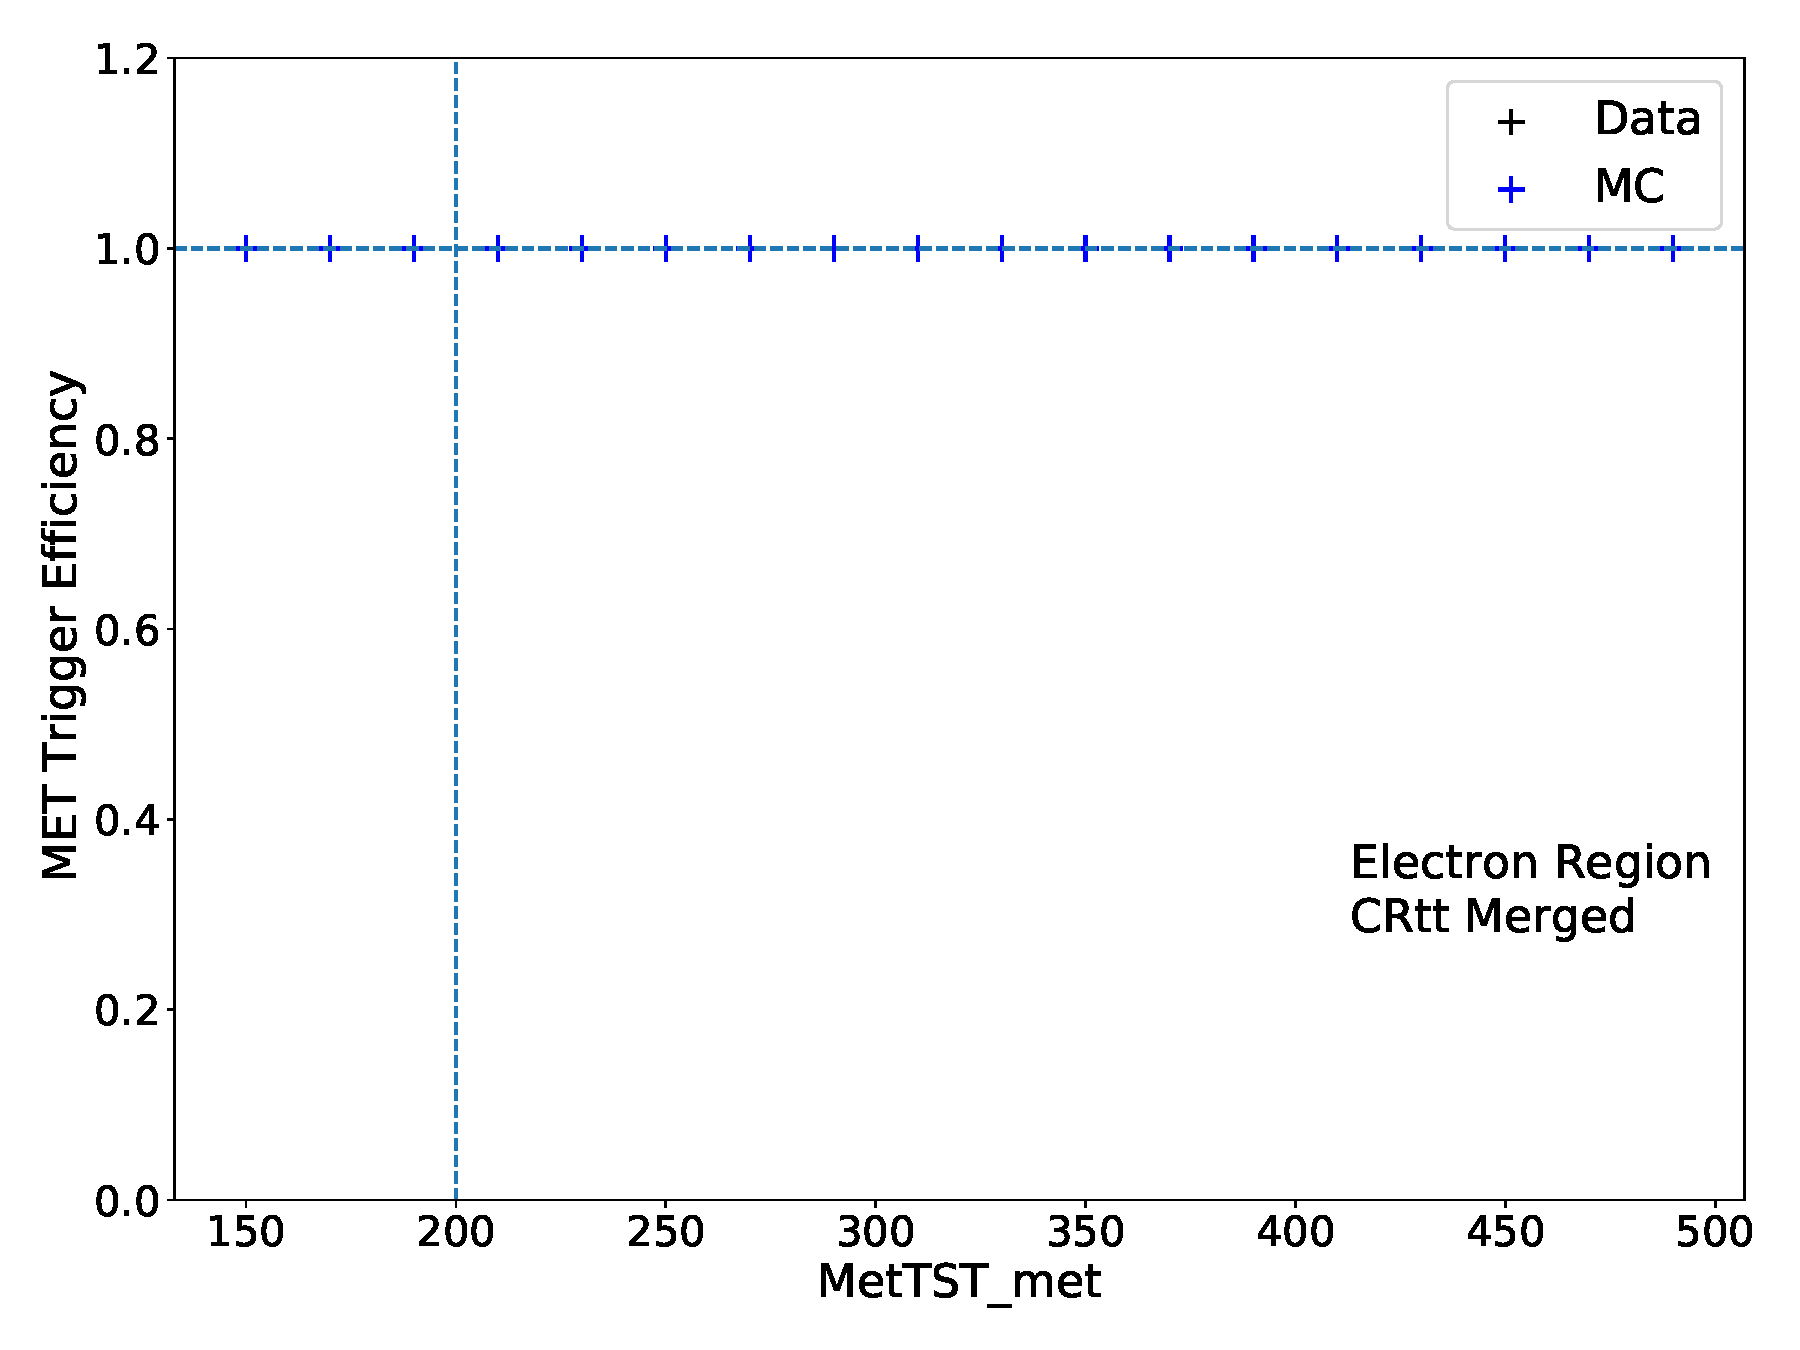
\includegraphics[width = 0.98\textwidth]{Figures/4/trig/trig_e/CRtt Merged/MetTST_met.pdf}
     \caption{\ttbar CR Merged}
     \end{subfigure}
     \begin{subfigure}{0.49\textwidth}
     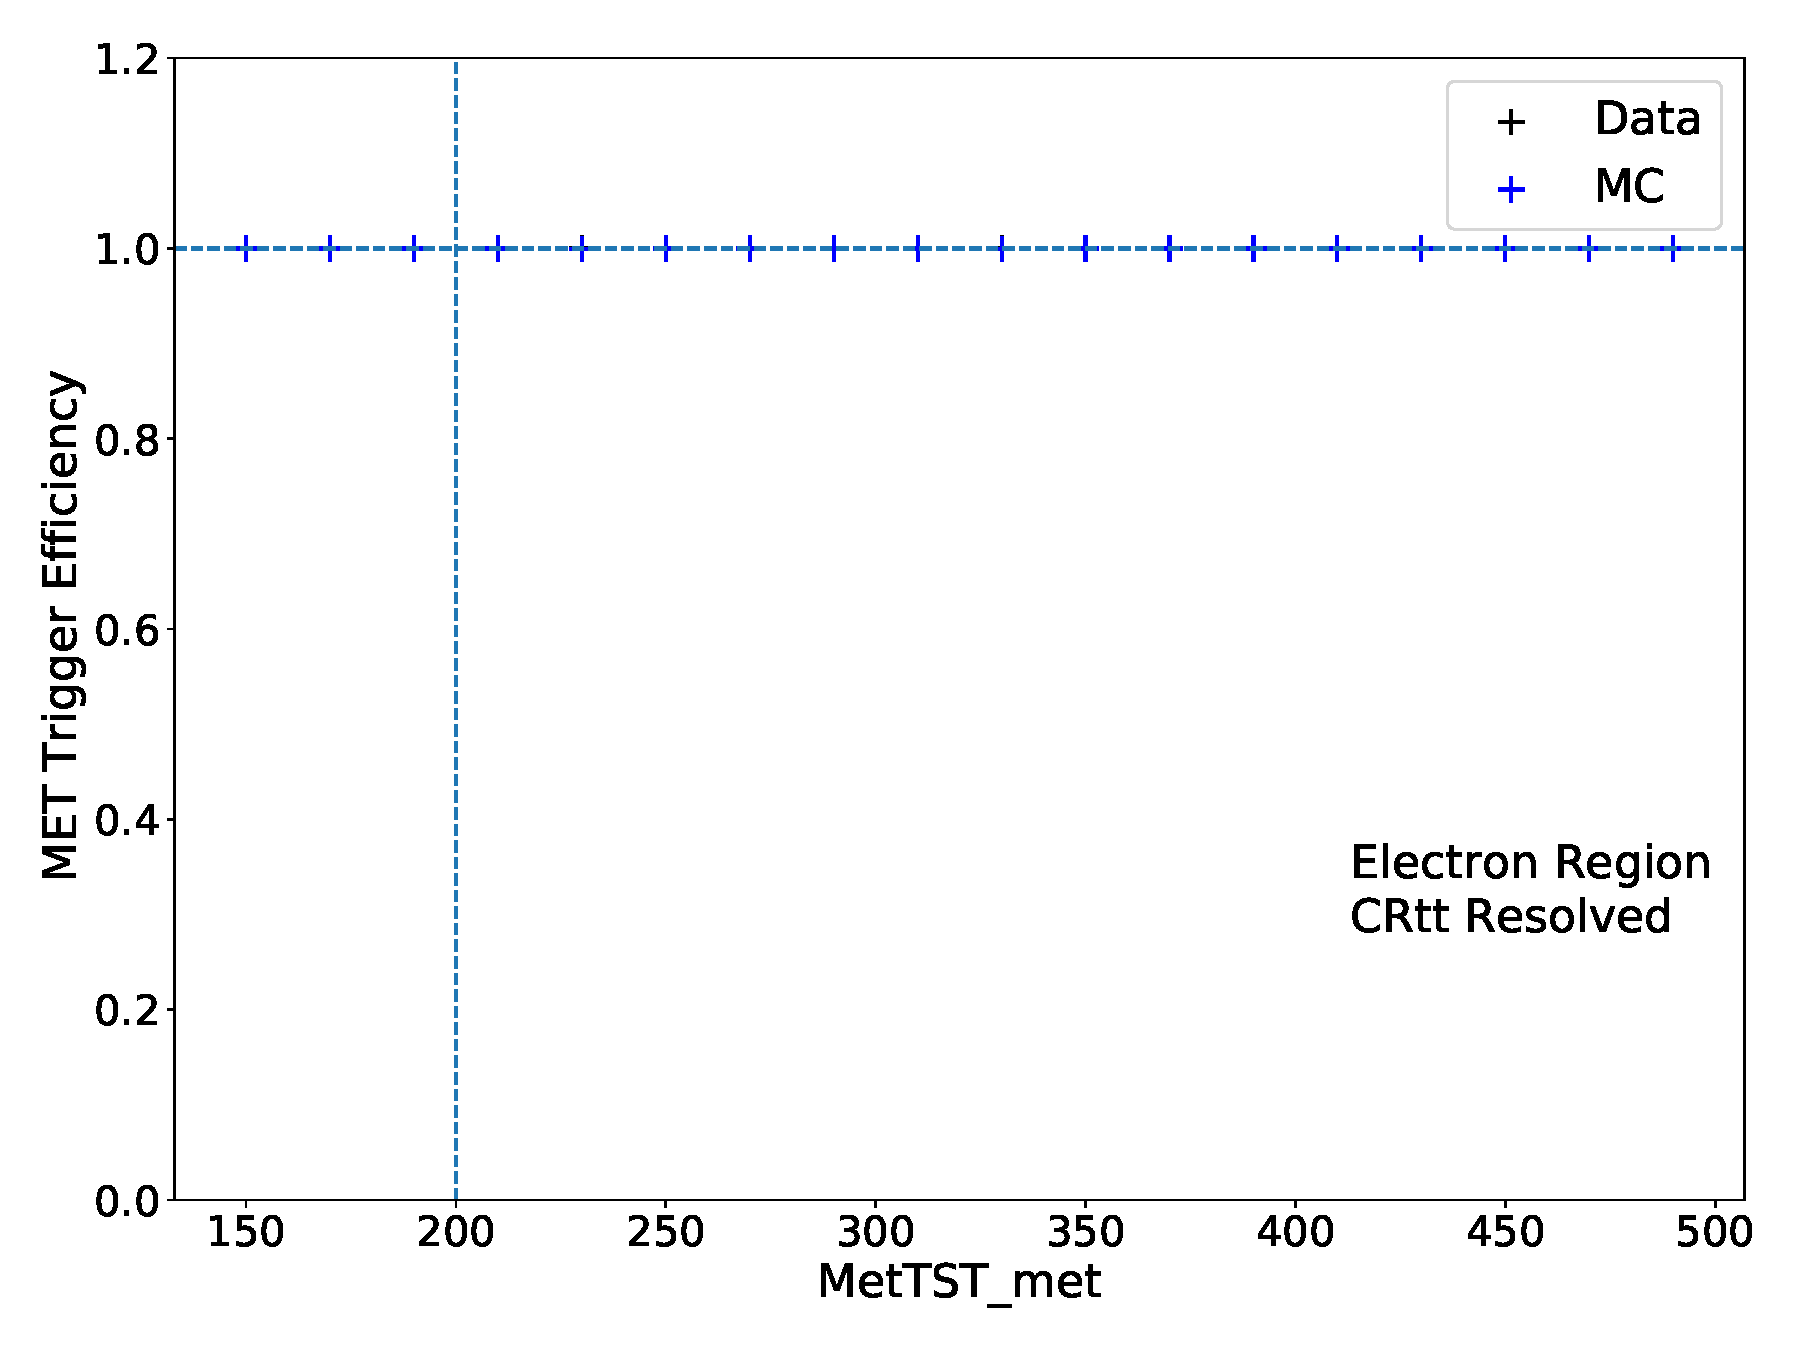
\includegraphics[width = 0.98\textwidth]{Figures/4/trig/trig_e/CRtt Resolved/MetTST_met.pdf}
     \caption{\ttbar CR Resolved}
     \end{subfigure}
  \caption{\met trigger efficiency in the electron channel.}
  \label{fig:trig_e}
\end{figure}

\begin{figure}[tb]
  \centering
     \begin{subfigure}{0.49\textwidth}
     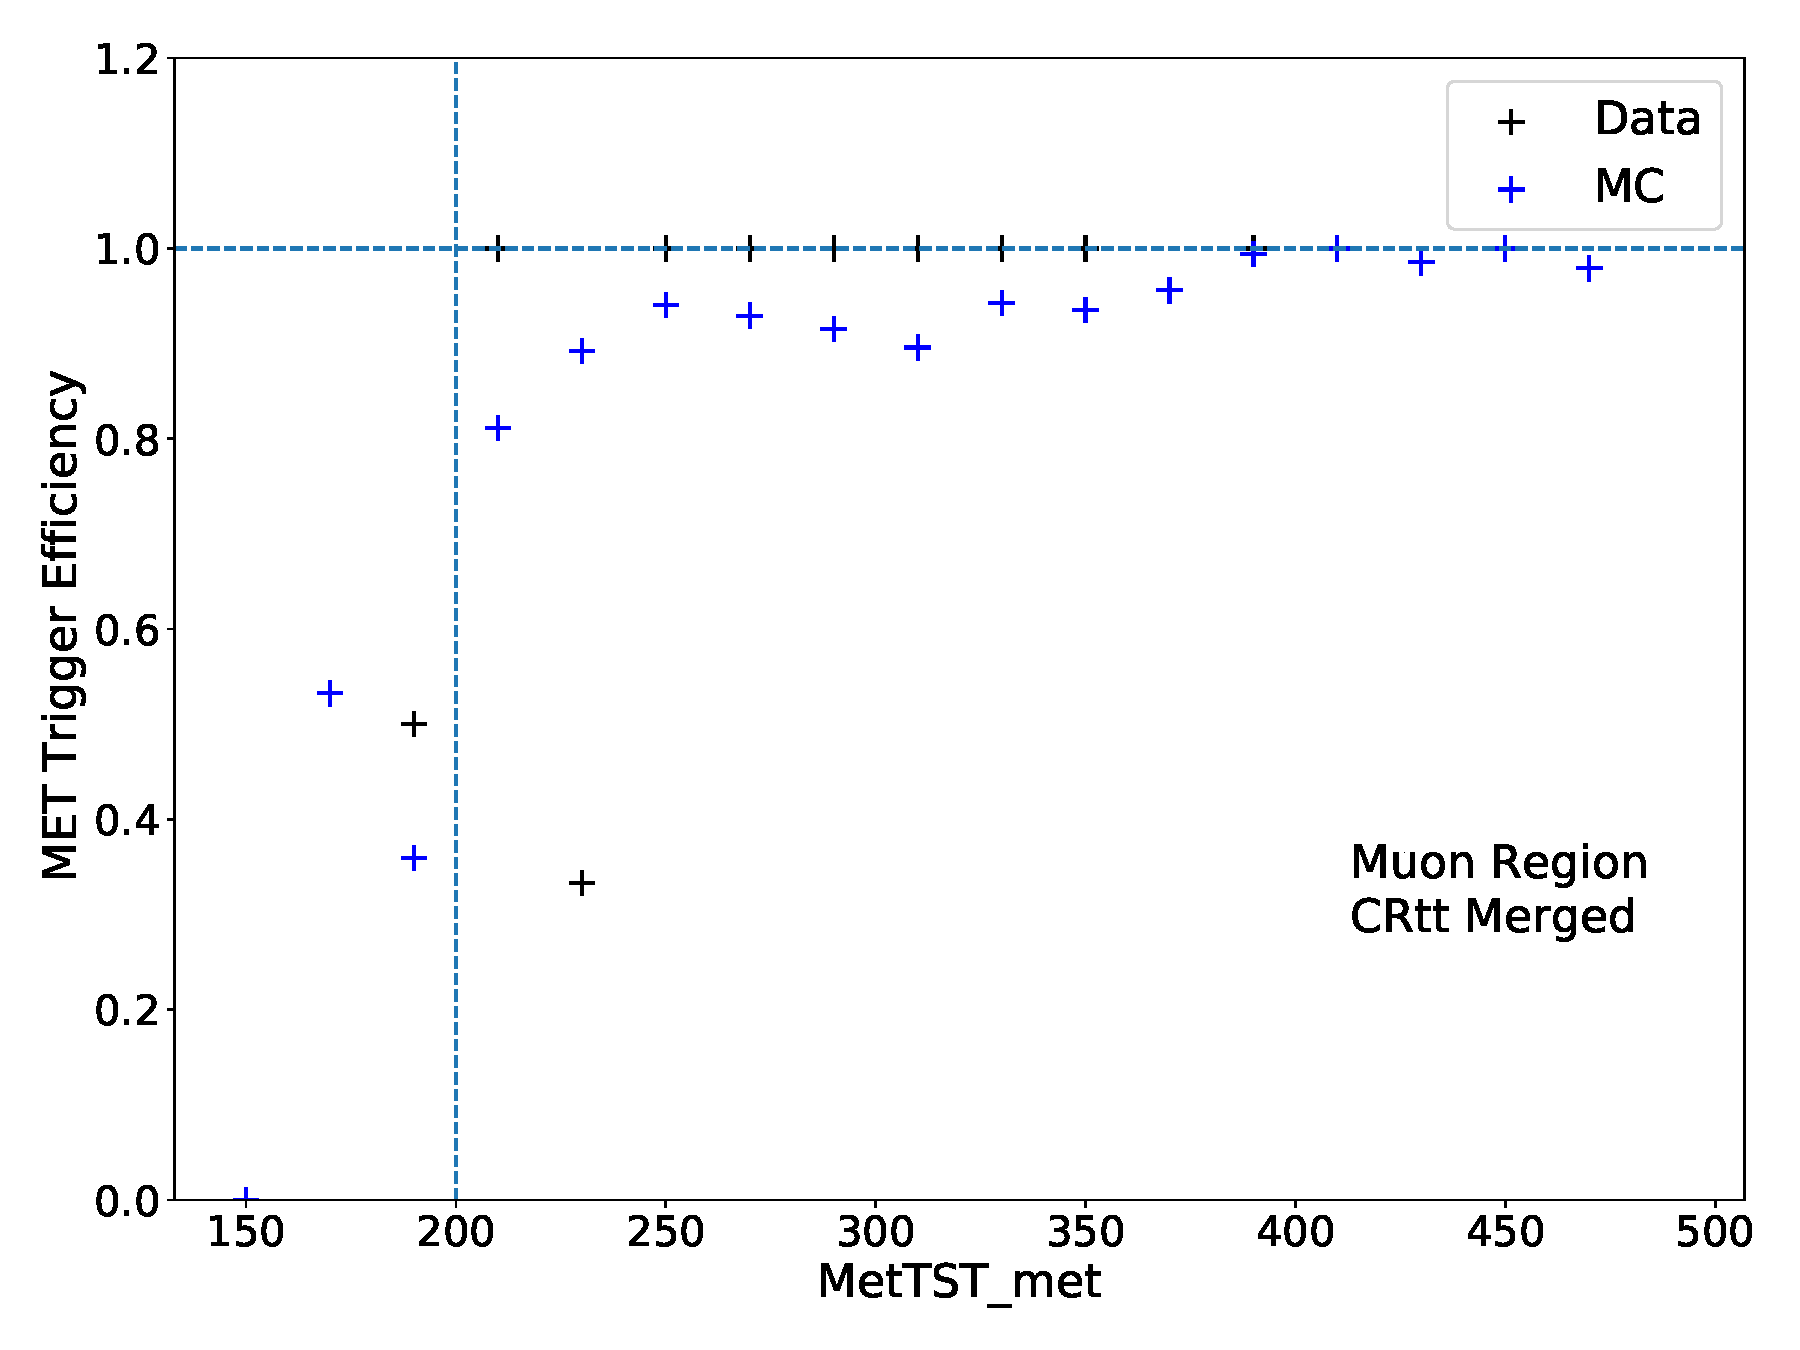
\includegraphics[width = 0.98\textwidth]{Figures/4/trig/trig_mu/CRtt Merged/MetTST_met.pdf}
     \caption{\ttbar CR Merged}
     \end{subfigure}
     \begin{subfigure}{0.49\textwidth}
     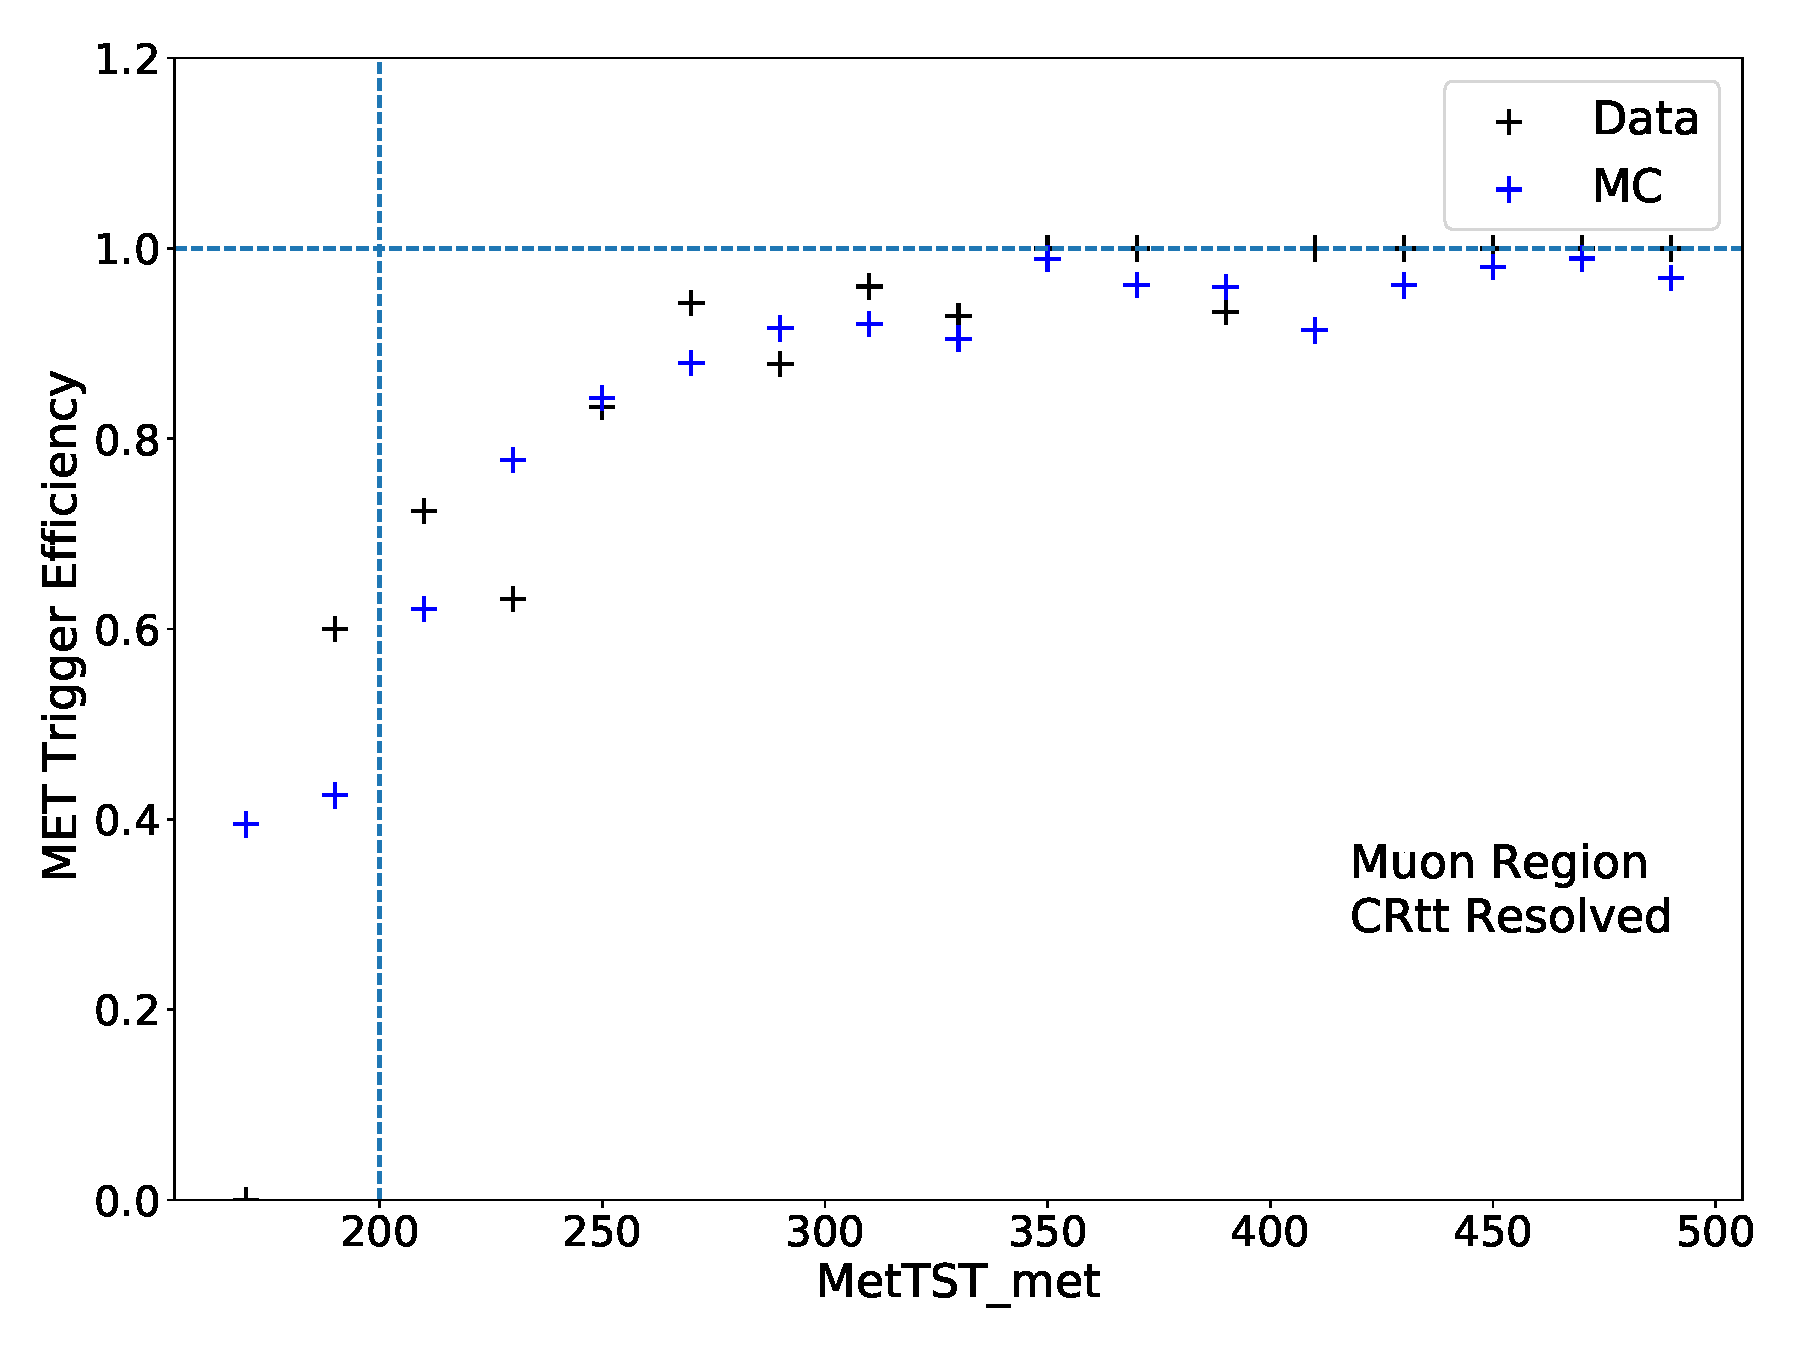
\includegraphics[width = 0.98\textwidth]{Figures/4/trig/trig_mu/CRtt Resolved/MetTST_met.pdf}
     \caption{\ttbar CR Resolved}
     \end{subfigure}
  \caption{\met trigger efficiency in the muon channel.}
  \label{fig:trig_mu}
\end{figure}

We hypothesized that the inefficiency was caused by high-\pT muons, which are not seen by the trigger-level \met calculation. As a result, if a muon travels in the opposite direction to the true \met, the measured trigger-level \met will be reduced and the trigger criteria may be failed. To confirm this, Figure \ref{fig:trig_invis} shows the \met trigger efficiency plotted against \met with signal muons treated as invisible (i.e. having their \pT subtracted from the \met).
In this case full or near-full trigger efficiency for \met $(\text{no} \mu) > 200$~GeV is recovered. We find it desireable to obtain full trigger efficiency in order to avoid the uncertainty associated with calculating trigger scale factors to match the trigger behaviour of data and MC events. Therefore, to counter the trigger inefficiency we moved to a logical OR between the unprescaled \met triggers and the single muon triggers in Table \ref{tab:mu_trigs}. This is designed to ensure that the events with a high-\pT muon that fail the \met trigger will pass the single muon trigger and be considered. Figure \ref{fig:trig_OR} shows that this recovers full trigger efficiency.

\begin{figure}[tb]
  \centering
     \begin{subfigure}{0.49\textwidth}
     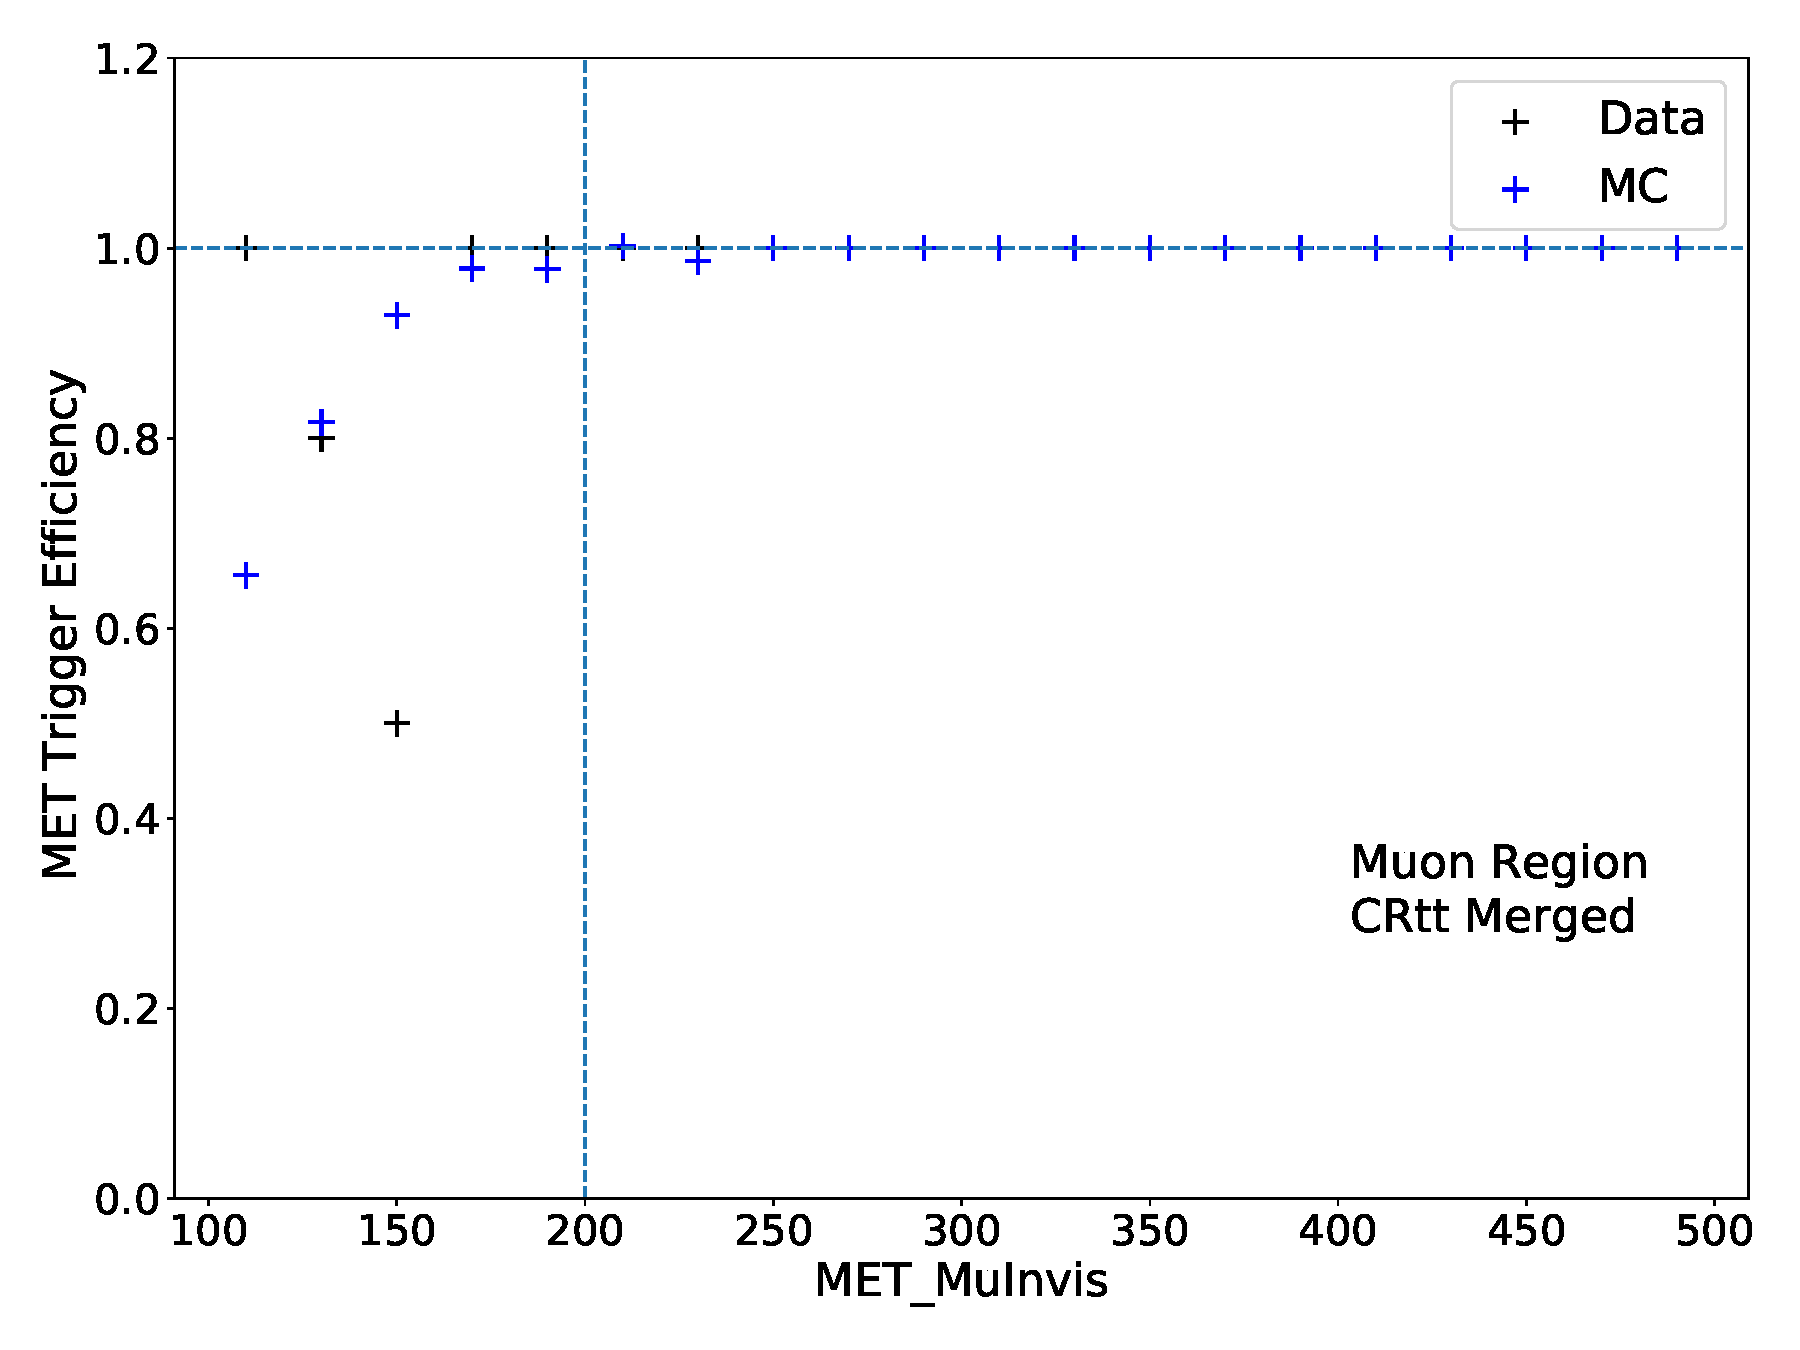
\includegraphics[width = 0.98\textwidth]{Figures/4/trig/trig_invis/CRtt Merged/MetTST_met.pdf}
     \caption{\ttbar CR Merged}
     \end{subfigure}
     \begin{subfigure}{0.49\textwidth}
     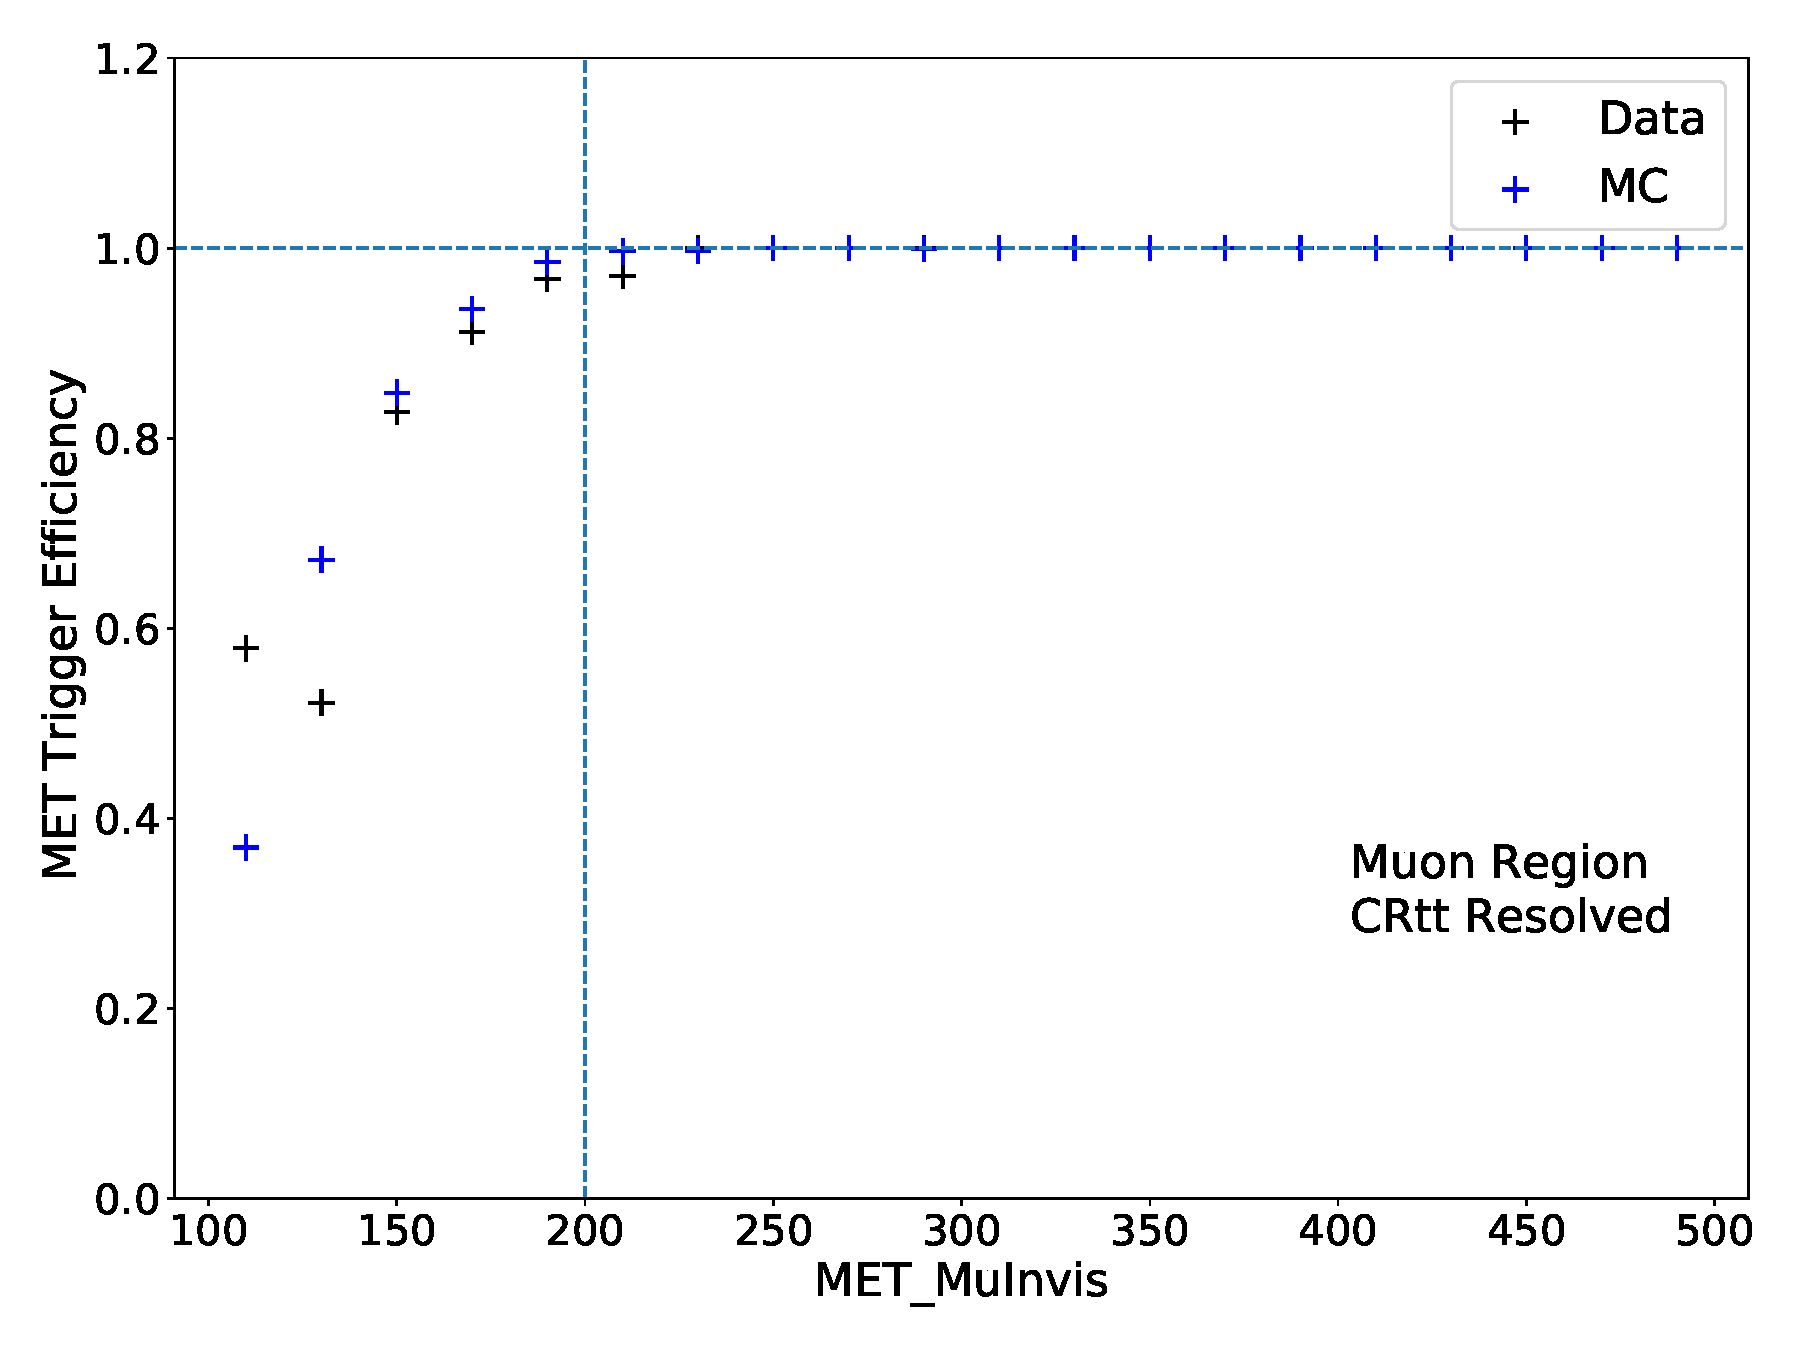
\includegraphics[width = 0.98\textwidth]{Figures/4/trig/trig_invis/CRtt Resolved/MetTST_met.pdf}
     \caption{\ttbar CR Resolved}
     \end{subfigure}
  \caption{\met trigger efficiency plotted against \met with muons invisible.}
  \label{fig:trig_invis}
\end{figure}

\begin{figure}[tb]
  \centering
     \begin{subfigure}{0.49\textwidth}
     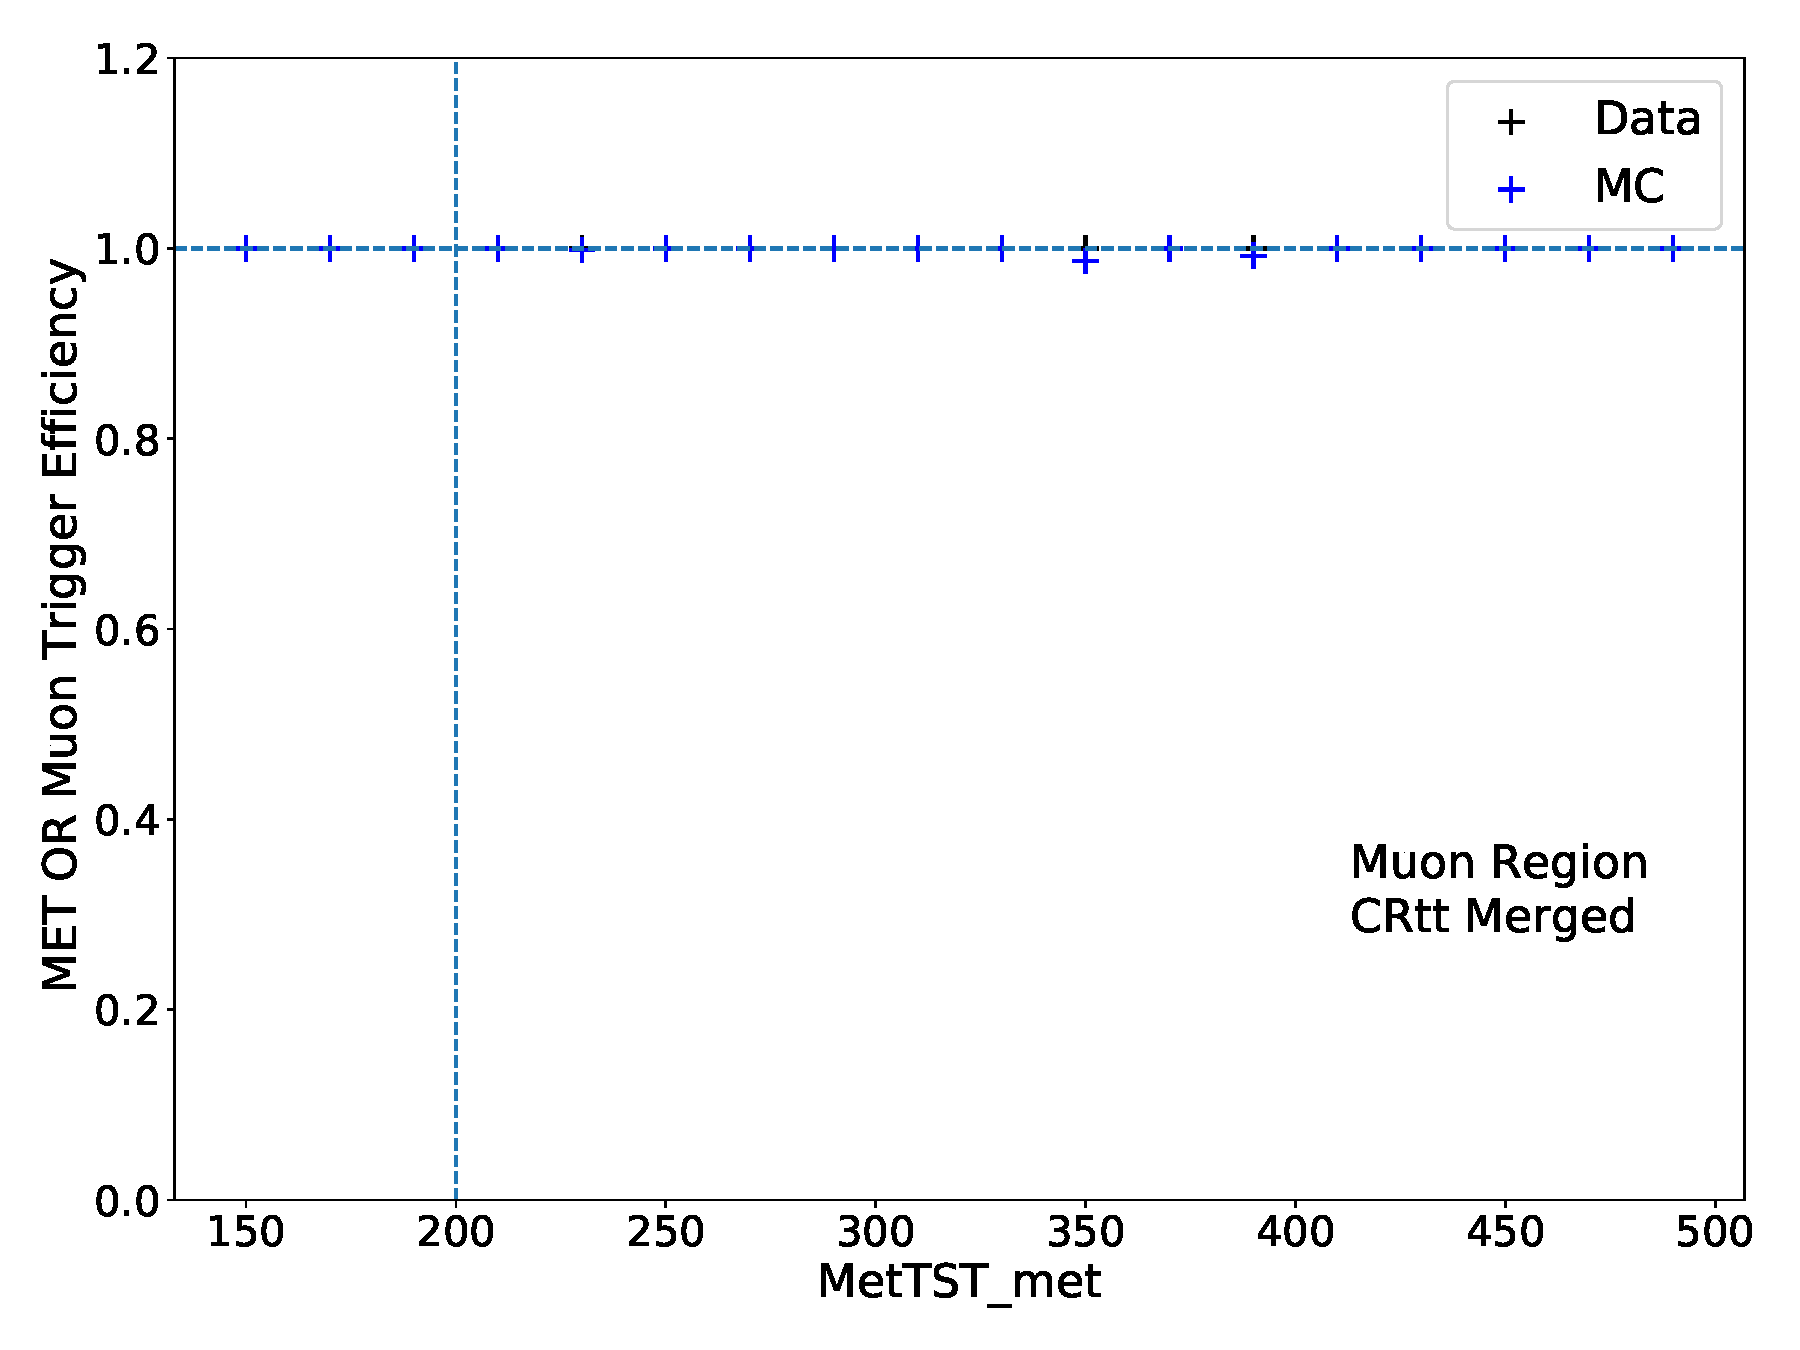
\includegraphics[width = 0.98\textwidth]{Figures/4/trig/trig_OR/CRtt Merged/MetTST_met.pdf}
     \caption{\ttbar CR Merged}
     \end{subfigure}
     \begin{subfigure}{0.49\textwidth}
     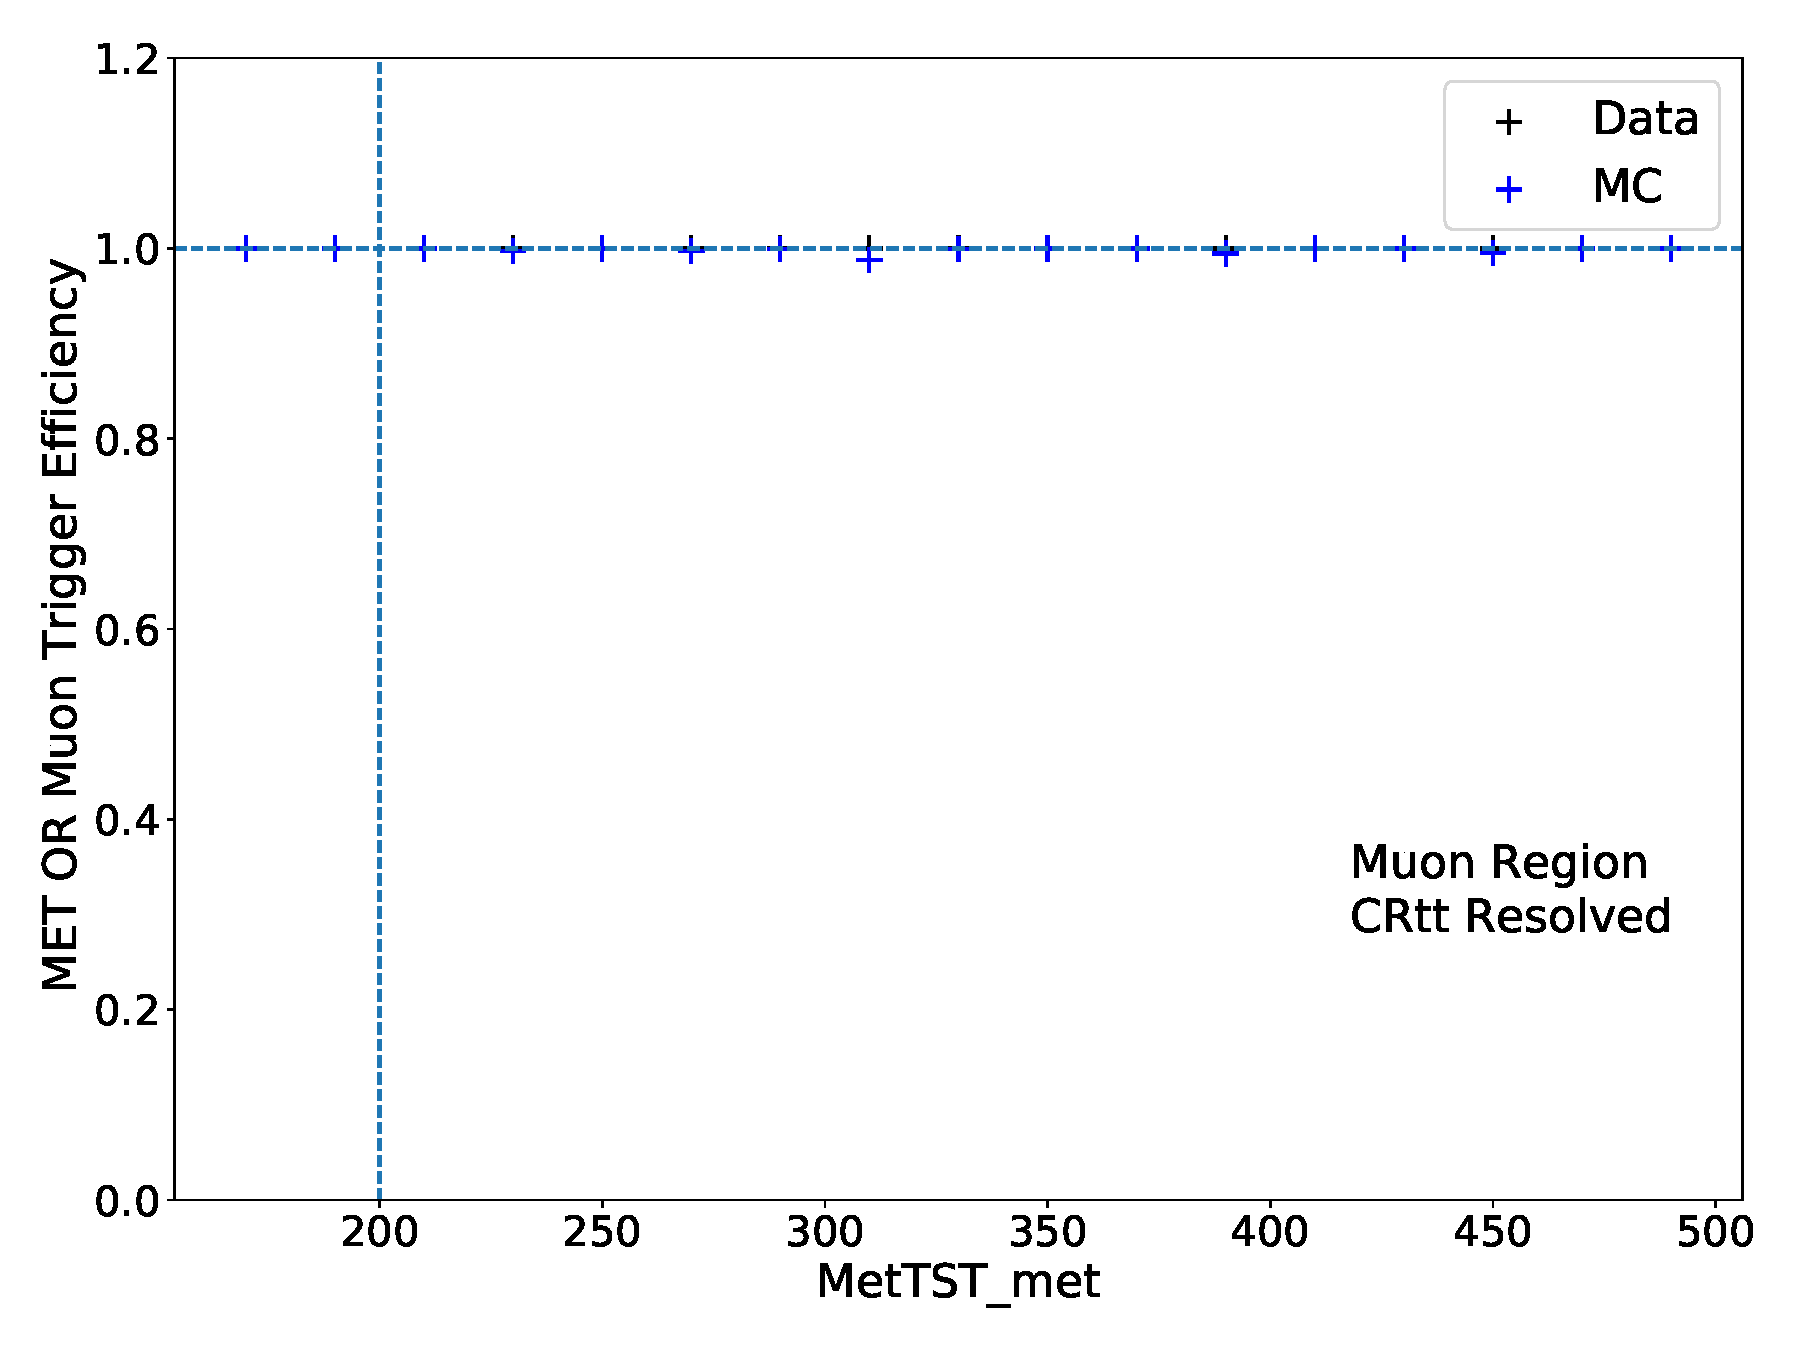
\includegraphics[width = 0.98\textwidth]{Figures/4/trig/trig_OR/CRtt Resolved/MetTST_met.pdf}
     \caption{\ttbar CR Resolved}
     \end{subfigure}
  \caption{Efficiency of the logical OR of \met and signle muon triggers.}
  \label{fig:trig_OR}
\end{figure}
